% 设定文章类型,正文字号为小四,若为五号将-4改为5即可
\documentclass[zihao=-4,UTF8]{report}		

% 文章宏定义

% \def\d{\mathrm{d}}
\def\p{\partial}

% 导入基本宏包
\usepackage[UTF8]{ctex}       % 设置文档为中文语言(中文paper留此行,删去上一行)
\usepackage{hyperref}   %(此宏包与标题中的数学环境冲突)  % 宏包:自动生成超链接
\usepackage{amsmath}    % 宏包:数学公式
\usepackage{amssymb}    % 宏包:提供更多数学符号
\usepackage{pifont}     % 宏包:提供了特殊符号和字体
\usepackage{extarrows}  % 宏包:更多箭头符号

%宏包:有色文本框及其设置
\usepackage[dvipsnames,svgnames]{xcolor}    %设置插入的文本框颜色
\usepackage[strict]{changepage}     % 提供一个 adjustwidth 环境
\usepackage{framed}     % 实现方框效果
\definecolor{graybox_color}{rgb}{0.95,0.95,0.96} % 文本框颜色。修改此行中的 rgb 数值即可改变方框纹颜色,具体颜色的rgb数值可以在网站https://colordrop.io/中获得。(截止目前的尝试还没有成功过,感觉单位不一样)(找到喜欢的颜色,点击下方的小眼睛,找到rgb值,复制修改即可)
\newenvironment{graybox}{%
\def\FrameCommand{%
\hspace{1pt}%
{\color{gray}\small \vrule width 2pt}%
{\color{graybox_color}\vrule width 4pt}%
\colorbox{graybox_color}%
}%
\MakeFramed{\advance\hsize-\width\FrameRestore}%
\noindent\hspace{-4.55pt}% disable indenting first paragraph
\begin{adjustwidth}{}{7pt}%
\vspace{2pt}\vspace{2pt}%
}
{%
\vspace{2pt}\end{adjustwidth}\endMakeFramed%
}

% 文章页面margin设置
\usepackage[a4paper]{geometry}
\geometry{top=1in}
\geometry{bottom=1in}
\geometry{left=0.75in}
\geometry{right=0.75in}   % 设置上下左右页边距
\geometry{marginparwidth=1.75cm}    % 设置边注距离(注释、标记等)

% 页眉页脚设置
\usepackage{fancyhdr}   %宏包:页眉页脚设置
\pagestyle{fancy}
\fancyhf{}
\cfoot{\thepage}
\renewcommand\headrulewidth{1pt}
\renewcommand\footrulewidth{0pt}
\chead{Thermodynamics Notes}    

% 标题自定义设置
\usepackage{titling}  % 宏包:标题设置

% 表格进阶设置
\usepackage{booktabs}
\usepackage{tabularx}
\usepackage{array}
\usepackage{longtable}

% 图表插入自定义设置
\usepackage{graphicx}  % 宏包:图片插入
\usepackage{float}     
\usepackage{caption}
\captionsetup[figure]{name=图}  % 设置图标题为“图”以防出现“figure”
\captionsetup[table]{name=表}   % 设置表标题为“表”以防出现“table”
\captionsetup{labelfont=bf, font=small}   % 将表、图等标题设置为bf,字号为small(五号)
\usepackage[export]{adjustbox}               

% 文章默认字体设置
\usepackage{fontspec}   % 宏包:更多字体种类
\usepackage{xcolor}    % 宏包:更多颜色设置
\setmainfont{SimSun}    % 设置中文字体为宋体字体
\setmainfont{Times New Roman} % 设置英文字体为Times New Roman

% 参考文献引用设置
\bibliographystyle{unsrt}   % 设置参考文献引用格式为unsrt
\newcommand{\upcite}[1]{\textsuperscript{\cite{#1}}}     % 自定义上角标式引用

% chapter标题自定义设置
\usepackage{titlesec}   
\titleformat{\chapter}[hang]{\normalfont\huge\bfseries\centering}{第\,\thechapter\,章}{20pt}{\Huge}
\titlespacing*{\chapter}{0pt}{-15pt}{20pt} % 控制上方空白的大小


% 文章序言设置
\newcommand{\enabstractname}{Abstract}
\newcommand{\cnabstractname}{序言}
\newenvironment{enabstract}{%
  \par\Large
  \noindent\mbox{}\hfill{\bfseries \enabstractname}\hfill\mbox{}\par
  \vskip 2.5ex}{\par\vskip 2.5ex}
\newenvironment{cnabstract}{%
  \par\Large
  \noindent\mbox{}\hfill{\bfseries \cnabstractname}\hfill\mbox{}\par
  \vskip 2.5ex}{\par\vskip 2.5ex}

% 文档作者信息设置
\title{\textbf{热学笔记\\Thermodynamics Notes}}
\author{丁毅\\ \footnotesize 中国科学院大学,北京 100049\\ Yi Ding \\ \footnotesize University of Chinese Academy of Sciences, Beijing 100049, China}
\date{\footnotesize 2024.1 - 2024.7}

 % 开始编辑文章
 \begin{document}
 \maketitle
 \newpage
 
 \addcontentsline{toc}{chapter}{序言} %手动添加为目录
 \thispagestyle{fancy}   %显示页码、页眉等
 \begin{cnabstract}
 {\normalsize 本书是笔者本科时的热学笔记,总结了热学学习中的主要知识,也有适当的拓展延伸。同时,对一些晦涩的物理概念或公式,给出了笔者的个人理解,以帮助读者阅读。}
 \end{cnabstract}
 \pagenumbering{Roman} %页码为大写罗马数字
 
 \newpage
 \addcontentsline{toc}{chapter}{目录}
 \tableofcontents
 \thispagestyle{fancy}
 
 \newpage
 \pagenumbering{arabic} 

\chapter{热力学系统}

\section{物质结构基本图象(略)}
\section{热力学系统及其状态参量}
\subsubsection{系统、环境:}
热力学研究对象的集合称为热力学系统,简称系统(system),除系统外的所有对象构成外界环境。\par
\ding{172}\ 开放(open):物质交换+能量交换\par
\ding{173}\ 绝热(adiabatic):物质交换\par
\ding{174}\ 封闭(closed):能量交换\par
\ding{175}\ 孤立(isolated):无
\subsubsection{状态参量:}
略。

\section{热力学平衡与热平衡}
\subsubsection{热力学平衡:}
\ding{172}\ 平衡态:在不受外界影响的条件下,系统各部分的宏观性质不发生任何变化。\par
\ding{173}\ 稳定态:在受到外界影响的条件下,系统各部分的宏观性质不发生任何变化。\par
\ding{174}\ 弛豫时间:系统由初态达到平衡态所需的时间。\par
{\color{gray}\small 热力学平衡要求力学平衡、化学平衡和热学平衡。热力学平衡是指一个系统达到某种平衡,热平衡是指两个或多个系统达到相同温度。}
\subsubsection{热接触:}
如果两个系统彼此只允许传递热量,而不允许发生相互作用或物质传递,此时称这两个系统彼此处于热接触。
\subsubsection{热平衡:}
如果将两个处于热力学平衡态的系统发生热接触时没有热量传递,也即达到相同温度,就称这两个系统处于热平衡状态。{\color{gray}\small 由于系统之间的对称性,热平衡应当具有反身性(自反性)和对称性。}

\section{温度与温标}
\subsubsection{温度:}
本质上,温度是组成系统的大量微观粒子的无规则运动剧烈程度的表现和度量。
\subsubsection{热力学第零定律(Zerot h Law of Thermodynamics):}
温度不同的两个系统发生通过热接触,最终会达到相同温度(热平衡),且宏观性质不再变化(分别达到热力学平衡)。\par
{\color{gray}\small 热力学第零定律提供了判断温度高低的基本原理,可据此发展出温标。}
\subsubsection{温标(temperature scale):}
测温物质、测温属性及曲线、固定标准点为温标三要素。\par
有经验温标(华氏、摄氏)、理想气体温标、热力学温标和国际实用温标。\par
华氏温标与摄氏温标转换:
\begin{equation}
    {\color{red} t_F = 32 + \frac{9}{5}t_C},\ \ \  t_C = \frac{5}{9}(t_F-32)
\end{equation}\par
理想气体温标与摄氏温标转换:
\begin{equation}
    {\color{red} T = 273.15 + t_C}
\end{equation}
\begin{table}[H]
    \centering
    \caption{常见温标数值}
    \begin{tabular}{ccccccccccc}
    \toprule
    名称 & 水的冰点 & 水的三相点 & 水的沸点\\
    \midrule
    摄氏温标 & 0 & 0.01 & 100\\
    理想气体温标& 273.15& 273.16 & 373.15\\
    \bottomrule
    \end{tabular}
\end{table}

\section{状态方程}

\subsubsection{状态方程的概念:}
处于平衡态的热力学系统的状态参量之间满足的一定的函数关系称为该热力学系统的状态方程,简称状态方程(equation of state,简记为EOS)。
\subsubsection{理想气体状态方程:}
\noindent
\begin{align}
    \text{单种气体:}&\ \  pV = \nu  RT\ \text{或}\ p = nkT\\
    \text{混合气体:}&\ \  (\sum p_i)V = (\sum \nu_i)RT \ \ \ \ {\color{gray}\text{可导出道尔顿分压定律}}
\end{align}
\indent {\color{gray}\small 其中$\nu =\frac{m}{M}$为气体物质的量,$n  = \frac{\mathrm{d}N}{\mathrm{d}V}$为分子数密度,$R=\frac{p_0V_m}{T_0}=8.31\ \mathrm{J/(mol\cdot K)}$为普适气体常量,$p_0$、$V_m$、$T_0$为气体在标准状态下的压强、摩尔体积、温度。在本笔记中,通常用$\nu$ 表示物质的量,用$n$表示气体的分子数密度。}

\subsubsection{范德瓦尔斯方程:}
对于范德瓦尔斯气体,其状态方程为:
\begin{equation}
    \left( p+a\cdot \frac{\nu ^2}{V^2} \right) \left( V-b \cdot \nu \right)  = \nu RT
\end{equation}
其中,$a = 4V_0\varepsilon_0N_A^2$(若分子间作用力为sutherland势),$b = 4N_AV_0$(b为p趋于无穷时气体所占据的体积)。
\subsubsection{位力展开和卡末林-昂尼斯方程:}
将宏观状态参量$p$与$T$的关系按摩尔浓度的幂次展开,则得到:
\begin{align*}
    pV_m =& A + \frac{B}{V_m} + \frac{C}{V_m^2} + \frac{D}{V_m^3}\cdots\\
    \text{或}&\\
    pV_m =& A + Bp + Cp^2 +Dp^3 + \cdots 
\end{align*}\par
这种表示实际气体的宏观状态参量之间关系的方法称为位力展开(virial expansion),所得的方程常称为卡末林—昂尼斯方程(Kamerlingh-Onnes equation),简称昂尼斯方程。\par
{\color{gray}\small 可以验证,范德瓦尔斯方程是特殊形式的具有更
清楚物理意义的昂尼斯方程}
\subsubsection{数学补充(偏微分):}
后面的知识需要用到偏微分,我们在此给出其理论基础。设函数$f(x,y,z) = 0$给出自变量$x,y,z$之间的隐函数关系(如$p,V,T$),则有:
\begin{align*}
    \frac{\partial x}{\partial y} = \frac{1}{\ \frac{\partial y}{\partial x} \ }\ \  ,\ \ \ \ 
    \frac{\partial x}{\partial y}\cdot \frac{\partial y}{\partial z}\cdot \frac{\partial z}{\partial x} = {\textcolor{red}{-1}}
\end{align*}
另外,当我们把函数$F = F(x,y)$写成$F = F(x,y(x,z)) = F(x,z)$时,由链式法则可以得到:
\begin{gather}
    \left(\frac{\partial f}{\partial x}\right)_z = \left(\frac{\partial f}{\partial x}\right)_y + \left(\frac{\partial f}{\partial y}\right)_x \left(\frac{\partial y}{\partial x}\right)_z \\
    \left(\frac{\partial f}{\partial z}\right)_x = \left(\frac{\partial f}{\partial x}\right)_y\left(\frac{\partial y}{\partial z}\right)_x
\end{gather}\par
{\color{gray}\small 当函数的变量是明显的,不需要特别说明时,我们不加以标注(没有括号的例子),而物理中变量的选取比较自由,因此我们常加以标注(有括号的例子)。}
\subsubsection{确定状态方程的唯象方法:}
\ding{172}\ 等压膨胀系数:
\begin{equation}
    \alpha = \frac{1}{V} \left( \frac{\partial V}{\partial T}\right)_p
\end{equation}\par
\ding{173}\ 
等体压强系数:
\begin{equation}
    \beta = \frac{1}{p}\left( \frac{\partial p}{\partial T}\right)_V
\end{equation}\par
\ding{174}\ 等温压缩系数:
\begin{equation}
    \kappa  = -\frac{1}{V}\left(\frac{\partial V}{\partial p} \right)_T
\end{equation}\par
且三者满足:
\begin{equation}
    p\beta \kappa = \alpha
\end{equation}

通过实验测出$\kappa,\alpha,\beta$关于$p,V,T$的函数关系后,可以通过求解微分方程得到系统的状态方程:\par
\ding{172}\ 已知$\beta,\kappa$:
\begin{equation}
    \frac{\mathrm{d}p}{p} = \beta\mathrm{d}T - \frac{1}{\kappa pV}\mathrm{d}V
\end{equation}\par
\ding{173}\ 已知$\alpha,\kappa$:
\begin{equation}
    \frac{\mathrm{d}V}{V} = \alpha \mathrm{d}T - \kappa \mathrm{d}p
\end{equation}\par
\ding{173}\ 已知$\alpha,\beta$:
\begin{equation}
    \mathrm{d}T = \frac{1}{\alpha V}\mathrm{d}V + \frac{1}{\beta p}\mathrm{d}p
\end{equation}

\section{理想气体初级微观理论}

\subsubsection{理想气体微观模型:}
研究气体必须建立合适的模型,对于理想气体模型,我们需要作出一些假设,或者说,满足如下条件的气体可以视为理想气体:\par
\ding{172}\ 气体分子大小远小于分子间的平均距离,可以忽略不计\par
\ding{173}\ 气体分子间距离很大,除碰撞瞬间外,分子间的相互作用力可以忽略不计\par
\ding{174}\ 分子间的碰撞、分子与器壁间的碰撞可以视为完全弹性碰撞\par
除上述假设外,还要对气体中分子的运动作出统计性假设:\par
对于大量气体分子来说,当气体处于平衡状态时,每一个分子沿各个方向运动的概率是相同的,即在任意时刻,沿各个方向运动的分子数目相等,这表明气体分子的速度沿各个方向的各种平均值相等(如算术平均数、几何平均数、平方平均数等),也即$\overline{v^2_x}=\overline{v^2_y}=\overline{v^2_z}$。如果这个假设不成立,则气体将集中在容器的某一部分,这与事实不符。

\subsubsection{理想气体压强公式:}\noindent
\begin{equation}
    p= \frac{1}{3}n \overline{Pv} 
    \label{理想气体压强公式}
\end{equation}\par
{\color{gray}\small 其中$P = m_0v$为单个分子的动量,考虑相对论效应时,$m_0$为分子动质量。}\par
特别地,对于非相对论气体,有:
\begin{equation}
    p = \frac{1}{3}nm_0\overline{v^2} = \frac{2}{3}n\overline{E_k} = \frac{1}{3}\rho \overline{v^2} 
\end{equation}\par
对于极端相对论气体,有:
\begin{equation}
    p = \frac{1}{3}n\overline{E_k} = \frac{1}{3}nm_0c^2
\end{equation}
\indent{\color{gray}\small 上面的$n = \frac{N}{V}$为分子数密度,$m_0$为一个分子的质量,$\rho = \frac{m}{V}$为气体质量密度,$k=\frac{R}{N_A}=1.38\times10^{-23}\ \mathrm{J/K}$为玻尔兹曼常量。}

\begin{graybox}
    \textbf{理想气体压强公式的推导:}\par
    如图\ref{理想气体压强公式推导},假设容器是长方体,各边长分别为$l_1$、$l_2$、$l_3$,容器中气体分子总数为$N$,每一个分子的质量为$m_0$。当气体处于平衡状态时,器壁各处压强相同,考虑器壁$A_1$面上的压强,取一个气体分子,假设其速度为$\boldsymbol{v}$,如图作速度分解,在$\mathrm{d}t$时间内,有:
    \begin{align*}
        F_0\mathrm{d}t
        &=2m_0v_y\ \ \text{\color{gray}\small (完全弹性碰撞、冲量定理)}\\
        \Longrightarrow F&=\sum_{i}^{} \frac{v_{iy}\mathrm{d}t}{2l_1}F_{i0}
        =\sum_{i}^{} \frac{v_{iy}}{2l_1}2m_0v_{iy}
        =\sum_{i}^{} \frac{m_0}{l_1}v_{iy}^2\\
        \Longrightarrow p&=\frac{F}{S}
        =\frac{m_0}{l_1l_2l_3}\sum_{i}^{}v_{iy}^2
        =\frac{Nm_0}{l_1l_2l_3}\overline{v_y^2}
        =\frac{m}{V}\overline{v_y^2}
        =\frac{1}{3}\rho \overline{v^2}
    \end{align*}
   \indent 特别地,可以证明,上式对任意容器成立。
\end{graybox}
\begin{figure}[H]
    \centering
    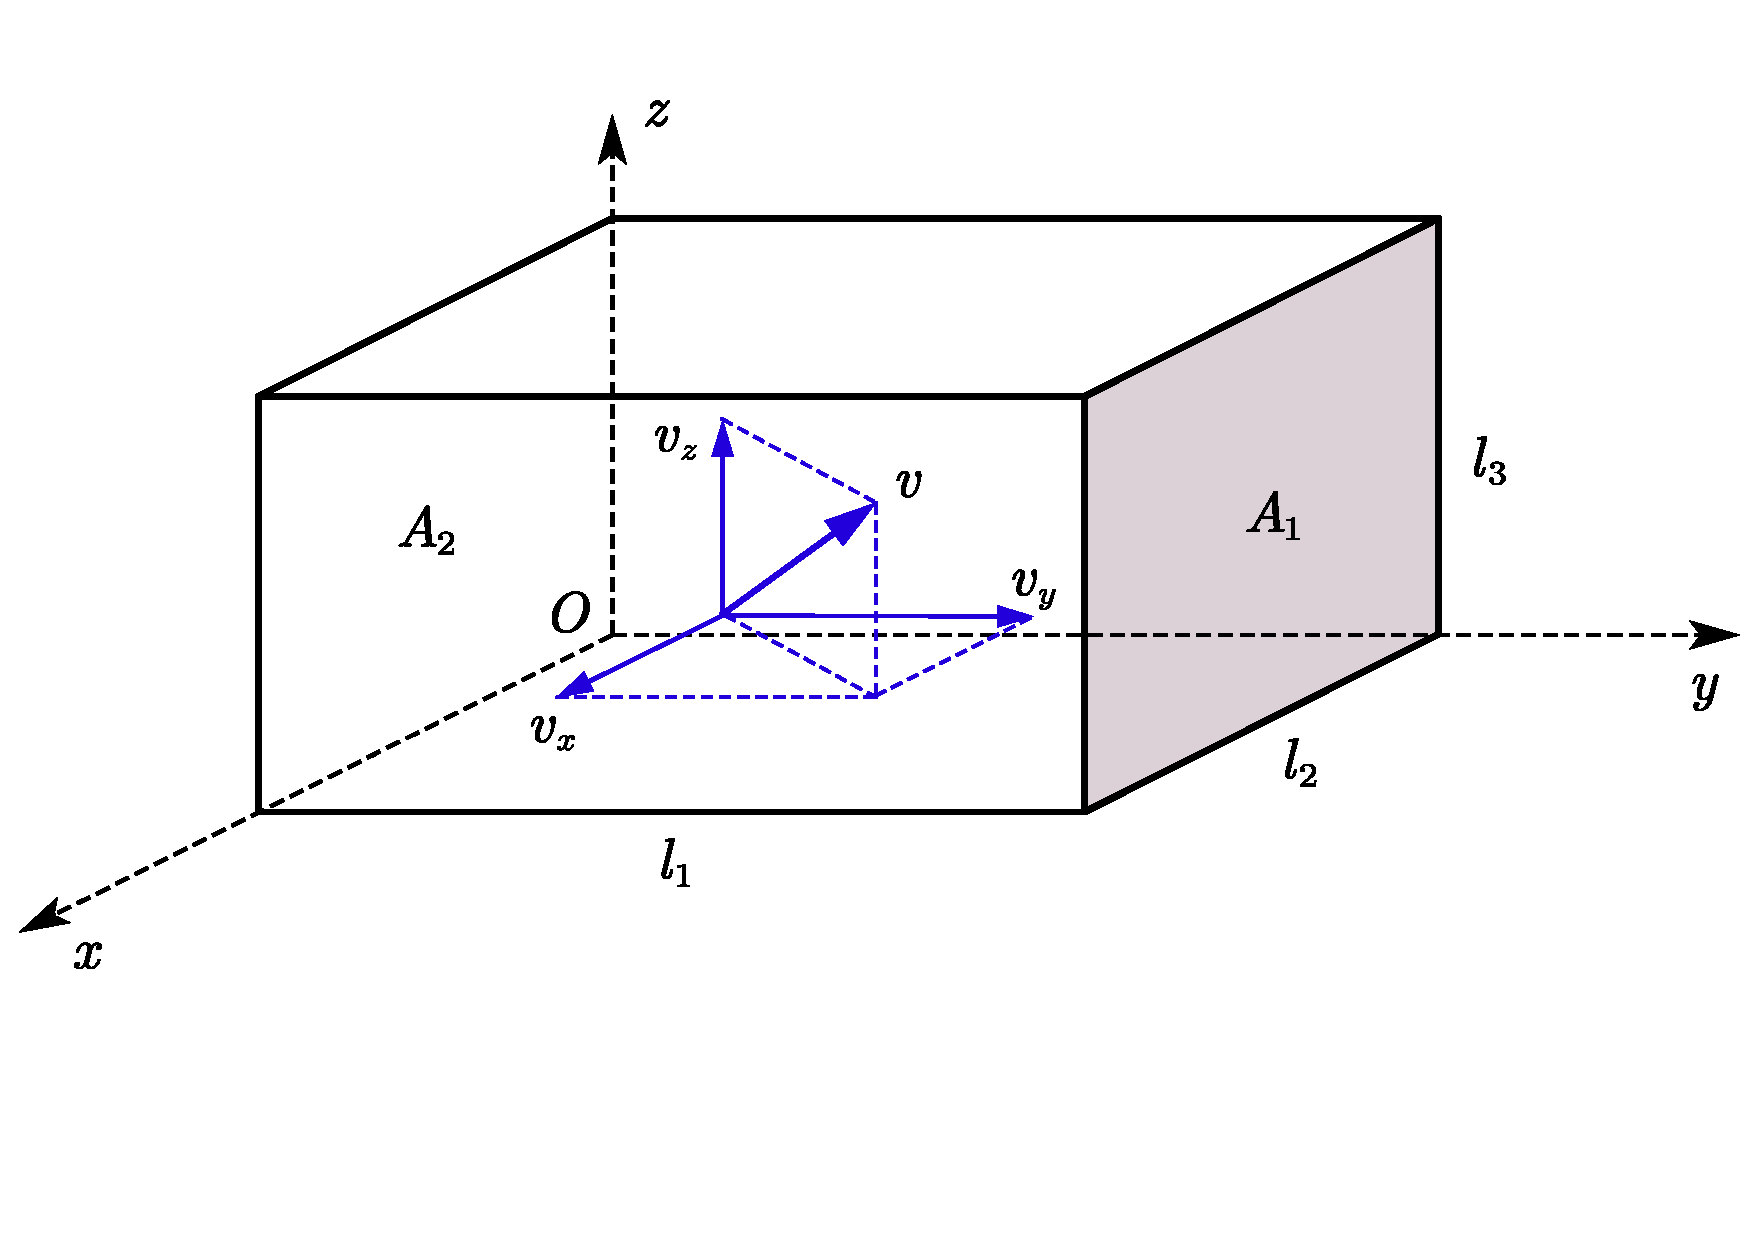
\includegraphics[width=0.7\textwidth]{pic/示意图一_crop.pdf}
    \caption{理想气体压强公式推导}
    \label{理想气体压强公式推导}
\end{figure}

\subsubsection{单原子气体平均动能:}
对大量单原子分子构成的气体而言,每一个分子自由度$i=3$,分子平均动能为:
\begin{align}
    &\text{非相对论气体:}\ \ \overline{E_k}=\frac{3}{2}kT\\
    &\text{纯相对论气体:}\ \ \overline{E_k}=E = 3kT
    \label{气体动能公式}
\end{align}

\begin{graybox}
    \textbf{单原子气体平均动能的推导:}
    \begin{align*}
        p=\frac{\nu RT}{V}= \frac{NRT}{N_AV}=\frac{N}{V}\frac{R}{N_A}T=nkT
        \overset{\text{公式}(\ref{理想气体压强公式})}{\Longrightarrow} \overline{E_k}=\frac{1}{2}m\overline{v^2}=\frac{3}{2}kT
    \end{align*}
    \indent 即得到公式(\ref{气体动能公式})。
\end{graybox}

\chapter{热平衡态下的统计分布律}

\section{统计规律与分布函数}
\subsubsection{事件及其概率:}
不相容事件具有归一性$\sum_{i} P(A_i) = 1$,且:
\begin{align}
    &\text{不相容事件:}\ \ P(A_i+A_j) = P(A_i) + P(A_j)\\
    &\text{独立事件:}\ \ P(A_i\cdot A_j) = P(A_i) \cdot P(A_j)
\end{align}
\subsubsection{分布函数:}
分布函数定义:
\begin{align}
    f(x) = \frac{1}{N}\frac{\mathrm{d}N}{\mathrm{d}x},\ \ \mathrm{d}P = f(x) \mathrm{d}x,\ \ \overline{x} = \int xf(x)\mathrm{d}x
\end{align}

\subsubsection{常见分布律:}
\ding{172}\ 平面无规行走:
\begin{equation}
    f(x,y) = Ce^{-\alpha (x^2+y^2)}
\end{equation}\par
\ding{173}\ 高斯分布(正态分布):
\begin{equation}
    f(x) = \frac{1}{\sigma \sqrt{2\pi }}e^{-\frac{1}{2}(\frac{x-\mu }{\sigma})^2}
\end{equation}\par
\ding{174}\ 二项式分布:
\begin{equation}
    \frac{\sqrt{\overline{(\Delta n_1)^2}}}{\overline{n_1}} = \frac{1}{\sqrt{N}}\sqrt{\frac{q}{p}}    
\end{equation}

\section{麦克斯韦分布律}
\subsubsection{高斯积分:}
后文的推导涉及高斯积分,公式如下:
\begin{equation}
    \int_{\textcolor{red}{-\infty}}^{+\infty}e^{-x^2}\mathrm{d}x = \sqrt{\pi}
\end{equation}
其它推论:
\begin{equation}
    G_0(\alpha) = \int_{\textcolor{red}{0}}^{+\infty} e^{-\alpha x^2}\mathrm{d}x = \frac{\sqrt{\pi }}{2}\cdot \frac{1}{\alpha^{\frac{1}{2}}}
\end{equation}
\begin{equation}
    G_1(\alpha) = \int_{\textcolor{red}{0}}^{+\infty} xe^{-\alpha x^2}\mathrm{d}x = \frac{1}{2}\cdot \frac{1}{\alpha^1}
\end{equation}
\begin{equation}
    G_2(\alpha) = \int_{\textcolor{red}{0}}^{+\infty} x^2e^{-\alpha x^2}\mathrm{d}x = \frac{\sqrt{\pi }}{4}\cdot \frac{1}{\alpha^{\frac{3}{2}}}
\end{equation}
\begin{equation}
    G_3(\alpha) = \int_{\textcolor{red}{0}}^{+\infty} x^3e^{-\alpha x^2}\mathrm{d}x = \frac{1}{2}\cdot \frac{1}{\alpha^2}
\end{equation}\par 
{\color{gray}\small 事实上,我们可以推导出:
\begin{gather}
    \int_{0}^{+\infty }x^{2n}e^{-\alpha x^2}\mathrm{d}x = \frac{(2n-1)!!}{2^{n+1}\alpha^n},\ \ \ \int_{0}^{+\infty} x^{2n+1}e^{-\alpha x^2}\mathrm{d}x = \frac{n!}{2\alpha^{n+1}}\\
    \int_{0}^{+\infty } \frac{x^a}{(1+x^b)^c}\mathrm{d}x = \frac{\Gamma(\frac{1+a}{b})\Gamma(c-\frac{1+a}{b})}{b\Gamma(c)}
\end{gather}\par
在考试时,只需要记得$x^0$,$x^1$,$x^2$分别对应$\frac{\sqrt{\pi}}{2}$,$\frac{1}{2}$,$\frac{\sqrt{ \pi}}{4}$即可。
}
\subsubsection{高斯分布:}
概率密度通常为高斯分布形式:
\begin{equation}
    f(x) = \frac{1}{\sigma\sqrt{2\pi }}e^{-\frac{1}{2}\left(\frac{x-\mu }{\sigma}\right)^2}
\end{equation}
{\color{gray}\small 概率密度$f$是概率分布$F$的导函数,有$F(X) = \int_{-\infty}^{X} f(t)\mathrm{d}t = P(x \le X)$。}
\subsubsection{麦克斯韦速\textcolor{red}{度}分布律:}
速度分布函数$f_M$是以$v_x,v_y,v_z$为轴的三维直角坐标系中的矢量函数,自变量为$\boldsymbol{v} = (v_x,v_y,v_z)$\ $ = v_x\boldsymbol{i} +v_y\boldsymbol{j}+v_z\boldsymbol{k}$\ :
\begin{equation}\textcolor{red}{f_M(\boldsymbol{v}) = \left(\frac{m_0}{2\pi kT}\right)^{\frac{3}{2}}e^{-\frac{m_0v^2}{2kT}} = \left(\frac{m_0}{2\pi kT}\right)^{\frac{3}{2}}e^{-\frac{E_k}{\,kT\,}}}
\end{equation}\par
一个粒子,速度在$[\boldsymbol{v} , \boldsymbol{v} + \mathrm{d}\boldsymbol{v}]$之间的概率,也即在$[v_x ,v_x +\mathrm{d}v_x]$,$[v_y ,v_y +\mathrm{d}v_y]$,$[v_z ,v_z +\mathrm{d}v_z]$之间的概率为:
\begin{equation}
    \mathrm{d} P =f_M(\boldsymbol{v})\mathrm{d}^3\boldsymbol{v}=f_M(\boldsymbol{v})\mathrm{d}v_x\mathrm{d}v_y\mathrm{d}v_z
\end{equation}

\subsubsection{麦克斯韦速\textcolor{red}{率}分布律:}
对速度分布函数进行球坐标中$\theta $和$\varphi$的二重积分(对相同速率的各个方向进行求和),得到速率分布函数:
\begin{equation}\textcolor{red}{ F_M(v) = 4\pi v^2 f_M(\boldsymbol{v}) }
   = 4\pi v^2\left(\frac{m_0}{2\pi kT}\right)^{\frac{3}{2}}e^{-\frac{m_0v^2}{2kT}} = 4\pi v^2\left(\frac{m_0}{2\pi kT}\right)^{\frac{3}{2}}e^{-\frac{E_k}{\,kT\,}}
\end{equation}\par

一个粒子,速率在$[v, v+\mathrm{d}v]$之间的概率为:
\begin{equation}
    \mathrm{d} P = F_M(v)\mathrm{d}v = 4\pi v^2\left(\frac{m_0}{2\pi kT}\right)^{\frac{3}{2}}e^{-\frac{m_0v^2}{2kT}}\mathrm{d}v
\end{equation}
\indent{\color{gray}\small 注:麦克斯韦速度分布律、麦克斯韦速率分布律为不考虑粒子间相互作用和外界对系统的作用所得到的结果。}\par
{\color{gray}\small  如图所示,$f(v)\mathrm{d}v$表示一个气体分子的速率在区间[$v$,\ $v+\mathrm{d}v$]内的概率,乘上$N$则表示所有气体分子中速率在[$v$,\ $v+\mathrm{d}v$]的分子数量。注意,麦克斯韦速度分布律是在分子间作用力可以忽略的情况下推得的,适用于理想气体,一些特殊气体(如高压、极低温气体)不再适用。}

\begin{figure}[H]
    \centering
    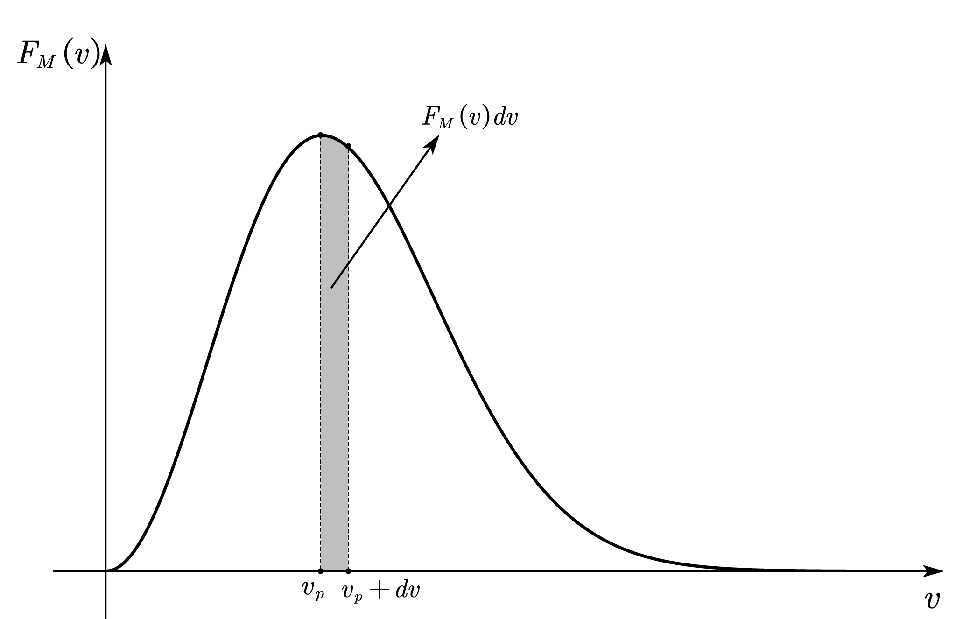
\includegraphics[width=0.7\textwidth]{pic/麦克斯韦速率分布函数.pdf}
    \label{麦克斯韦速率分布图}
\end{figure}
\begin{graybox}
    \textbf{麦克斯韦速率分布函数的推导:}\par
    设$f$表示速度分布函数,$F$表示速率分布函数。设$v_x$,$v_y$,$v_z$表示粒子速度在三维直角坐标系下的速度分量。由微观粒子各向同性、宏观静止可以判断,速度分布仅与$\boldsymbol{v}$的大小有关,与方向无关,于是存在函数$g$使得
    \begin{equation}
        f(\boldsymbol{v}) = g(\boldsymbol{v}^2) = g(v_x^2,v_y^2,v_z^2)
    \end{equation}
    又$v_x$,$v_y$,$v_z$相互独立,于是:
    \begin{equation}
        g(v_x^2,v_y^2,v_z^2) = g(v_x^2)g(v_y^2)g(v_z^2)\Longrightarrow \ln g(v^2) = \ln g(v_x^2) + \ln g(v_y^2)+\ln g(v_z^2)
    \end{equation}
    仿照无规行走的思路,作试探解$\ln g(v_i^2) = A-Bv_i^2$,$i = x,y,z$,可以得到:
    \begin{equation}
        f(\boldsymbol{v}) = g(v^2) = Ce^{-B(v_x^2 + v_y^2 +v_z^2)} = Ce^{-Bv^2}
    \end{equation}
    其中$B$,$C$为待定常量,可由分布函数归一性、能量守恒联立解出。在球坐标系中,作如下积分:
    \begin{gather}
        \int f(\boldsymbol{v})\mathrm{d}^3\boldsymbol{v} = \int_{0}^{+\infty} \int_{2\pi}^{0}\int_{\pi}^{0} Ce^{-Bv^2}v^2\sin \theta \mathrm{d}v\mathrm{d}\theta\mathrm{d}\varphi = 1\\
        \int (\frac{1}{2}m_0v^2)f(\boldsymbol{v})\mathrm{d}^3\boldsymbol{v} = \frac{m_0}{2}\int_{0}^{+\infty} \int_{2\pi}^{0}\int_{\pi}^{0} v^2Ce^{-Bv^2}v^2\sin \theta \mathrm{d}v\mathrm{d}\theta\mathrm{d}\varphi = \frac{3}{2}kT
    \end{gather}
    借助高斯积分知识求解,可以得到$B = \frac{m_0}{2kT}$,$C = \left(\frac{m_0}{2\pi kT}\right)^{\frac{3}{2}}$,因此得:
    \begin{equation}
        f(\boldsymbol{v}) = \left(\frac{m_0}{2\pi kT}\right)^{\frac{3}{2}}e^{-\frac{m_0v^2}{2kT}}
    \end{equation}
    将$f(\boldsymbol{v})\mathrm{d}^3\boldsymbol{v}$对角度$\theta$和$\varphi$积分,去掉方向因素,得到粒子速率在$[v,v+\mathrm{d}v]$之间的概率$F(v)\mathrm{d }v$:
    \begin{align*}
        F(v)\mathrm{d}v &= \int f(\boldsymbol{v})\mathrm{d}^3\boldsymbol{v} \\
        &= \int_{0}^{2\pi } \int_{0}^{\pi }  f(\boldsymbol{v})v^2\sin \theta  \mathrm{d}v\mathrm{d}\theta\mathrm{d}\varphi\\
        & = 4\pi v^2 f(\boldsymbol{v})\mathrm{d}v \\
        \Longrightarrow  F(v) & = 4\pi v^2\left(\frac{m_0}{2\pi kT}\right)^{\frac{3}{2}}e^{-\frac{m_0v^2}{2kT}}
    \end{align*}
事实上,可以从$4\pi v^2$为球表面积的角度来理解$F(v) = 4\pi v^2 f(\boldsymbol{v})$。
\end{graybox}  
\subsubsection{平均速率:}
速率在$[v_1,v_2]$之间的粒子,$v$的平均值为:
\begin{equation}
    \overline{v} = \frac{\text{此区间分子速率总和}}{\text{此区间分子数}} = \frac{\int_{v_1}^{v_2}NvF(v)\mathrm{d}v }{\int_{v_1}^{v_2}NF(v)\mathrm{d}v} = \frac{\int_{v_1}^{v_2}vF(v)\mathrm{d}v }{\int_{v_1}^{v_2}F(v)\mathrm{d}v}
\end{equation}
类似的,$\varphi(v)$的平均值为:
\begin{equation}
    \overline{\varphi(v)} = \frac{\text{此区间分子速率总和}}{\text{此区间分子数}} = \frac{\int_{v_1}^{v_2}N\varphi(v)F(v)\mathrm{d}v }{\int_{v_1}^{v_2}NF(v)\mathrm{d}v} = \frac{\int_{v_1}^{v_2}\varphi(v)F(v)\mathrm{d}v }{\int_{v_1}^{v_2}F(v)\mathrm{d}v}
\end{equation}
\subsubsection{三种特殊速率:}
\ding{172}\ 最慨然速率:
麦克斯韦速率分布函数$F_M(v)$的极大值称为最慨然速率,用$v_p$表示。
\begin{equation}
    v_p = \sqrt{\frac{2kT}{m_0}} = \sqrt{\frac{2RT}{\mu }}
\end{equation}\par
{\color{gray}\small 这对应着$\varepsilon = \frac{1}{2}mv_p^2 = kT$}\par
\ding{173}\ 平均速率(算术平均数):粒子速率的算术平均值称为平均速率。
\begin{equation}
    \overline{v} = \int_{0}^{+\infty} vF_M(v)\mathrm{d}v = \sqrt{\frac{8kT}{\pi m_0}}
\end{equation}\par
\ding{174}\ 方均根速率(平方平均数):粒子速率的平方平均值称为方均根速率,记为$v_{rms}$。
\begin{equation}
    v_{rms} = \sqrt{\overline{v^2}} =  \sqrt{\int_{0}^{+\infty} v^2F_M(v)\mathrm{d}v} = \sqrt{ \frac{3kT}{m_0}} = \sqrt{ \frac{3RT}{\mu }}
\end{equation}\par    
{\color{gray}\small 这与$\overline{E_k} = \frac{3}{2}kT$所得的结果完全相同。}
\subsubsection{不同维度的麦克斯韦分布律:}
在不同维度中(一维,二维,三维),麦克斯韦分布律的表达式不同,但麦克斯韦速度分布律的分量式都符合:
\begin{equation}
    f(v_i) = \sqrt{\frac{m_0}{2\pi kT}}e^{-\frac{\varepsilon_{i}}{kT}}
\end{equation}\par
其中$i = x,y,z$,再根据$x,y,z$方向上的独立性,可以求出各个维度上的麦克斯韦速度分布律,进而求得速率分布律。\par
{\color{gray}\small 例如二维时,$f_M(\boldsymbol{v}) = f(v_x)f(v_y)$,且$F_M(v) = 2\pi vf_M(\boldsymbol{v})$。} 

\subsubsection{分子数密度关于速度(率)的分布:}
速度在$[\boldsymbol{v},\boldsymbol{v}+\mathrm{d}\boldsymbol{v}]$之间的分子,其分子数密度分布(依速度)、分子数密度分布(依速率)分别为:
\begin{align}
    n(\boldsymbol{v}) &= n f_M(\boldsymbol{v})\\
    n(v)& = n F_M(v)
\end{align}\par
且有关系$ = \int n(\boldsymbol{v})\mathrm{d}\boldsymbol{v} = \int n(v)\mathrm{d}v$。

\subsubsection{泻流数率:}
粒子束流从某个小孔射出的现象称为泻流,单位时间内射出单位面积小孔的粒子数称为泻流数率,记作$\Gamma$。\par
在三维中,小孔(狭缝)的线度远小于分子平均自由程时,有:
\begin{gather}\label{三维薄壁容器泻流数率}
    \textcolor{red}{j = nv_x} \Longrightarrow \mathrm{d}\Gamma = [nf(v_x)\mathrm{d}v_x]v_x  = nv_xf(v_x)\mathrm{d}v_x \overset{\text{积分}}{=}  nv_xf_M(\boldsymbol{v})\mathrm{d}\boldsymbol{v}\\
    \Longrightarrow \Gamma = \int_{\textcolor{red}{v_0}}^{+\infty} nv_xf(v_x)\mathrm{d}v_x = \textcolor{red}{\frac{1}{4}n\overline{v}\cdot e^{-(\frac{v_0}{v_p})^2}}
\end{gather}\par
对于“小孔”的线度极大的情况(例如天体大气溢出问题),上式不再成立,更正后有:
\begin{gather}
    \mathrm{d}\Gamma = \frac{1}{2}v \left[ nF_M(v)\mathrm{d}v\right] 
    \Longrightarrow \Gamma = \frac{1}{2}n\int_{v_0}^{+\infty}vF_M(v)\mathrm{d}v = \frac{n}{\sqrt{\pi}}\left[1+\left(\frac{v_0}{v_p}\right)^2\right]e^{-\left(\frac{v_0}{v_p}\right)^2}
\end{gather}\par
其中$v_0$为逃逸速度,$v_p =  \sqrt{\frac{2kT}{m}} $为最慨然速率,$\overline{v} = \sqrt{\frac{8kT}{\pi m}}$为平均速率。

\begin{graybox}
    \textbf{泻流数率的推导:}\\
    速度在$[\boldsymbol{v},\boldsymbol{v}+\mathrm{d}\boldsymbol{v}]$间的粒子,其数密度为$ nf_M(\boldsymbol{v})\mathrm{d}\boldsymbol{v}$,将这些粒子的速度都视为$\boldsymbol{v}$。先固定$v_x$不动,然后对于任意给定的$v_y$,$v_z$,都有一个圆柱,其中的粒子即为$\mathrm{d}t$时间内通过$\mathrm{d}S$的粒子,粒子数为:
    \begin{align*}
        \mathrm{d}\Gamma\mathrm{d}t \mathrm{d}S&= \left[n(\boldsymbol{v})\mathrm{d}^3\boldsymbol{v}\right]\left[(v_x\mathrm{d}t)\mathrm{d}S\right]\\
        \Longrightarrow  \mathrm{d}\Gamma &= n v_xf_M(\boldsymbol{v})\mathrm{d}v_x\mathrm{d}v_y\mathrm{d}v_z = n\cdot[v_xf(v_x)\mathrm{d}v_x]\cdot[f(v_y)\mathrm{d}v_y]\cdot[f(v_z)\mathrm{d}v_z]\\
        \Longrightarrow \Gamma 
        &= n \left[\int_{0}^{+\infty}v_xf_M(v_x)\mathrm{d}v_x \right] \cdot \left[\int_{-\infty}^{+\infty}  f_M(v_y)\mathrm{d}v_y\right]\cdot \left[\int_{-\infty}^{+\infty} f_M(v_z)\mathrm{d}v_z\right]\\
        & = n \int_{0}^{+\infty}v_xf_M(v_x)\mathrm{d}v_x = \frac{1}{4}n  \overline{v}
    \end{align*}
也可以像下面这样:\\
建立法向$x$轴后,粒子是否溢出仅与$v_x$有关,与其它无关。考虑\textcolor{red}{溢出数率公式$j = nv_x$},对于$x$方向速度在$[v_x, v_x + \mathrm{d}v_x]$之间的粒子,其数密度为$nf(v_x)\mathrm{d}v_x$,贡献的泻流数率$ \mathrm{d}\Gamma $为:
\begin{equation}
    \mathrm{d}\Gamma = [nf(v_x)\mathrm{d}v_x]v_x = n v_xf(v_x)\mathrm{d}v_x \Longrightarrow \Gamma = \int_{0}^{+\infty} n v_xf_M(v_x)\mathrm{d}v_x = \frac{1}{4}n  \overline{v} 
\end{equation}
\end{graybox}

\subsubsection{狭缝溢出的速率、速度分布:}
记$i$维狭缝速度分布为$f_{i}(\boldsymbol{v})$,$i$维狭缝速率分布为$F_{i}(v)$。在三维中,“狭缝”即为小孔(2维),在二维中,“狭缝”为一维,我们有结论:\par
\ding{172}\ 二维:
\begin{equation}
    f_2(\boldsymbol{v})\frac{2}{\sqrt{\pi}} \left(\frac{m}{2kT}\right)^{\frac{3}{2}}v_xe^{-\frac{mv^2}{2kT}}, \ \ F_2(v) = \frac{4}{\sqrt{\pi}}\left(\frac{m}{2kT} \right)^{\frac{3}{2}}v^2e^{-\frac{mv^2}{2kT}}
\end{equation}
\par
\ding{173}\ 三维:
\begin{equation}
    f_3(\boldsymbol{v}) = \frac{2}{\pi} \left( \frac{m}{2kT}\right)^2 v_x e^{\frac{mv^2}{2kT}}\ ,\ \ F_3(v) = 2\left(\frac{m}{2kT} \right)^2 v^3 e^{-\frac{mv^2}{2kT}} = \textcolor{red}{\frac{v}{\,\overline{v}\,}\cdot F_{M,3}(v)}
\end{equation}
\begin{graybox}
\textbf{泻流速度分布、速率分布的推导:}\\
记$i$维麦克斯韦速度分布为$f_{M,i}(\boldsymbol{v})$,$i$维麦克斯韦速率分布为$F_{M,i}(v)$,首先有结论,无论二维还是三维,有泻流数率:
\begin{equation}
    \Gamma =  n \int_{0}^{+\infty}v_xf_M(v_x)\mathrm{d}v_x =nK =n \sqrt{\frac{kT}{2\pi m}}
\end{equation}
也即记$K = \sqrt{\frac{kT}{2\pi m}}$,其中$m$为单个气体分子的质量(同教材一致),对于速度分布,其定义式为$f_i(\boldsymbol{v}) \mathrm{d}\boldsymbol{v} = \frac{\mathrm{d}N}{N}$,于是:\\ \textbf{(1)二维情况:}\\
$\mathrm{d}t$时间内通过狭缝$\mathrm{d}l$的总粒子数:
\begin{equation}
    N = \Gamma \mathrm{d}t\mathrm{d}l
\end{equation}
在这些粒子中,速度介于$[\boldsymbol{v},\ \boldsymbol{v} + \mathrm{d}\boldsymbol{v} ]$之间的有(利用圆柱体分析法):
\begin{align*}
    \mathrm{d}N & = \left[ n(\boldsymbol{v})\mathrm{d}\boldsymbol{v}  \right]\cdot \left[ v_x \mathrm{d}t\mathrm{d}l \right]\\
    & = \left[ nf_{M,2}(\boldsymbol{v})\mathrm{d}\boldsymbol{v}  \right]\cdot \left[ v_x \mathrm{d}t\mathrm{d}l \right]
\end{align*}
于是得到速度分布:
\begin{equation}
    f_2(\boldsymbol{v}) = \frac{nv_xf_{M,2}(\boldsymbol{v})}{\Gamma} = \frac{v_x}{K}f_{M,2}(\boldsymbol{v}) = \frac{1}{K}\cdot \frac{m}{2\pi kT}\cdot v_xe^{-\frac{m(v_x^2 + v_y^2)}{2kT}} = \frac{2}{\sqrt{\pi}} \left(\frac{m}{2kT}\right)^{\frac{3}{2}}v_xe^{-\frac{mv^2}{2kT}}
\end{equation}
在极坐标系中积分,可得速率分布,坐标转换为$v_x = v \cos \theta$,$v_y = v \sin \theta$。考虑到$v_x \ge 0 $,有$\theta \in [-\frac{\pi}{2}, \frac{\pi}{2}]$,于是:
\begin{align*}
    F_2(v)\mathrm{d}v 
    & = \int f_2(\boldsymbol{v}) \mathrm{d}\boldsymbol{v}
     = \int_{-\frac{\pi}{2}}^{\frac{\pi}{2}}f_2(\boldsymbol{v}) v \mathrm{d}\theta \mathrm{d}v 
    =   \int_{-\frac{\pi}{2}}^{\frac{\pi}{2}} \frac{v_x}{K}f_{M,2}(\boldsymbol{v}) v \mathrm{d}\theta \mathrm{d}v  \\
    & = \int_{-\frac{\pi}{2}}^{\frac{\pi}{2}} \frac{1}{K}f_{M,2}(\boldsymbol{v}) v^2 \cos \theta \mathrm{d}\theta \mathrm{d}v 
    = \frac{1}{K}f_{M,2}(\boldsymbol{v}) v^2 \mathrm{d}v \cdot \left[ \int_{-\frac{\pi}{2}}^{\frac{\pi}{2}}  \cos \theta \mathrm{d}\theta\right]\\
     &= \frac{2}{K}f_{M,2}(\boldsymbol{v}) v^2 \mathrm{d}v  = 4\pi \left( \frac{m}{2\pi kT}\right)^{\frac{3}{2}}v^2e^{-\frac{mv^2}{2kT}} \mathrm{d}v \\
    \Longrightarrow
    F_2(v) & = \frac{4}{\sqrt{\pi}}\left(\frac{m}{2kT} \right)^{\frac{3}{2}}v^2e^{-\frac{mv^2}{2kT}} 
\end{align*}
\textbf{(2)三维情况:}\\
同理有:
\begin{align*}
&N = \Gamma\mathrm{d}t\mathrm{d}S \ ,\ \ \mathrm{d}N = [n(\boldsymbol{v})\mathrm{d}\boldsymbol{v}]\cdot [v_x\mathrm{d}t\mathrm{d}S] = \left[ nf_{M,3}(\boldsymbol{v})\mathrm{d}\boldsymbol{v}  \right]\cdot \left[ v_x \mathrm{d}t\mathrm{d}S \right]\\
\Longrightarrow & f_3(\boldsymbol{v}) = \frac{v_x}{K}f_{M,3}(\boldsymbol{v}) = \frac{1}{K}\cdot \left(\frac{m}{2\pi kT} \right)^{\frac{3}{2}}\cdot v_xe^{-\frac{m(v_x^2 + v_y^2 + v_z^2)}{2kT}}
 = \frac{2}{\pi} \left( \frac{m}{2kT}\right)^2 v_x e^{\frac{mv^2}{2kT}}\end{align*}
在球坐标系中积分,可得速率分布,坐标转换为$v_x = v \sin\theta \cos \phi$,$v_x = v \sin\theta \sin \phi$,$v_z = v\cos \theta$。考虑到$v_x \ge 0 $,有$\phi \in [-\frac{\pi}{2}, \frac{\pi}{2}]$,于是:
\begin{align*}
    F_3(v)\mathrm{d}v 
    &=  \iint f_3(\boldsymbol{v}) \mathrm{d}\boldsymbol{v} 
    = \iint \frac{v_x}{K}f_{M,3}(\boldsymbol{v}) \mathrm{d}\boldsymbol{v}  
    = \iint \frac{v_x}{K}f_{M,3}(\boldsymbol{v}) \mathrm{d}v_x\mathrm{d}v_y\mathrm{d}v_z\\
    & = \iint \frac{v_x}{K}f_{M,3}(\boldsymbol{v})v^2 \sin \theta \mathrm{d}\theta \mathrm{d}\phi \mathrm{d}v  
    = \iint \frac{1}{K}f_{M,3}(\boldsymbol{v}) v^3 \sin^2 \theta \cos \phi \mathrm{d}\theta \mathrm{d}\phi \mathrm{d}v  \\
    &= \frac{1}{K} f_{M,3}(\boldsymbol{v})v^3\mathrm{d}v \cdot \left[ \int_{-\frac{\pi}{2}}^{\frac{\pi}{2}} \cos \phi \mathrm{d}\phi\right] \cdot \left[\int_{0}^{\pi}\sin^2 \theta  \mathrm{d} \theta\right] \\
    &= \frac{1}{K} f_{M,3}(\boldsymbol{v})v^3\mathrm{d}v \cdot 2 \cdot \frac{\pi}{2}  = 2 \left(\frac{m}{2kT} \right)^2 v^3 e^{-\frac{mv^2}{2kT}} \mathrm{d}v\\
    \Longrightarrow  F_3(v) &= 2 \left(\frac{m}{2kT} \right)^2 v^3 e^{-\frac{mv^2}{2kT}} 
\end{align*}\noindent
\end{graybox}

\subsubsection{黑体辐射热流密度:}

\begin{equation}
    j = \frac{\mathrm{d}Q}{\mathrm{d}S\mathrm{d}t} = \sigma T^4
\end{equation}\par
{\color{gray}\small 其中$\sigma$为 Stefan-Boltzmann 常量。}
\section{力场中的气体分布}

\subsubsection{重力场中的气体分布(等温):}
假设重力场中的气体可以视为理想气体,\textcolor{red}{且整个大气等温},我们有:
\begin{equation}
    n = n_0e^{-\frac{m_0gh}{kT}},\ \ \ \   p = p_0e^{-\frac{m_0gh}{kT}}
\end{equation}
\begin{graybox}
    \textbf{重力场气体分布推导:}\\
    取气体微元,底面积$\mathrm{d}S$,高$\mathrm{d}h$,用$n = n(h)$表示高为$h$处的分子数密度,有力学平衡:
    \begin{equation}
        (p+\mathrm{d}p)\mathrm{d}S - p\mathrm{d}S + (m_0n\mathrm{d}S\mathrm{d}h)g = 0
    \end{equation}
    化简得到:
    \begin{equation}
        \mathrm{d}p = - \rho g\mathrm{d}h = - nm_0g\mathrm{d}h
    \end{equation}
    联立理想状态方程$p = nkT$消去$n$,得到:
    \begin{equation}
        \frac{1}{p}\mathrm{d}p = -\frac{m_0g}{kT}\mathrm{d}h \Longrightarrow p = p_0e^{-\frac{m_0gh}{kT}}
    \end{equation}
\end{graybox}
\subsubsection{玻尔兹曼分布律:}
对任意无旋力场(可以建立势能与位矢的函数),设气体在$\boldsymbol{r}$处的势能为$E_p(\boldsymbol{r})$,则有玻尔兹曼(位置)分布律:
\begin{equation}
    n_B(\boldsymbol{r}) = n_0e^{-\frac{E_p}{kT}}
\end{equation}\par
其中,$\boldsymbol{r} = \boldsymbol{r_0}$时,$n_B(\boldsymbol{r})= n_0$ ,$E_p(\boldsymbol{r}) = 0$,即为所选取的参考点(也是势能零点)。\par
空间中,微元$\mathrm{d}V$内含有的分子数为:
\begin{equation}
    \mathrm{d}N = n\mathrm{d}V = n_0e^{-\frac{E_p}{kT}}\mathrm{d}x\mathrm{d}y\mathrm{d}z
\end{equation}
{\color{gray}\small 上式表明,力场中的气体分子总是优先占据势能较低的状态。}
\subsubsection{麦克斯韦-玻尔兹曼分布律:}
将微观粒子按速度的分布(麦克斯韦速度分布律)和按位置的分布(玻尔兹曼分布律)相结合:
\begin{equation}
    f_{MB}(\boldsymbol{v},\boldsymbol{r} ) =f_M(\boldsymbol{v})f_B(\boldsymbol{r})= C_0\left(\frac{m_0}{2\pi kT}\right)^{\frac{3}{2}}e^{-\frac{E_k + E_p}{kT}}
\end{equation}\par
可以证明,上式中的动能$E_k$可以是平动、振动、转动等各种形式运动的动能(结合即为内能$U$),势能$E_p$也不仅包括平直空间中势能,还包括其它各种形式的力场势能,因此,麦克斯韦-玻尔兹曼分布律(此后将简称为玻尔兹曼分布律)可以讨论任意经典热力学系统的性
质。

\section{能量均分定理}
\subsubsection{分子的自由度:}
由$n$个原子构成的分子最多有$3n$个自由度($3$平动,$3$转动,$3n-6$振动)。
设分子有$t$个平动自由度、$r$个转动自由度和$s$个振动自由度,则总自由度为:
\begin{equation}
    i = t + r + 2s
\end{equation}\par
\ding{172}\ 单原子分子:$t = 3,\ r = 0,\ s = 0$\par
\ding{173}\ 刚性双原子分子:$t = 3,\ r = 2,\ s = 0$\par
\ding{174}\ 非刚性双原子分子:$t = 3,\ r = 2,\ s = 1$\par
\ding{175}\ 刚性多原子分子:$t = 3,\ r = 3,\ s = 0$\par
另外,量子理论表明,同一分子的自由度并非一成不变,而是随着温度升高被逐渐“激发”。在经典热力学中,我们不必追究更深的物理本质,只需认为$t$,$r$,$s$在不同的温度下可能有不同的取值。
激发平动、转动、振动的特征温度分别为:
\begin{equation}
    T_1 = 10^{-12}\ \mathrm{K},\ \ T_2 = 100\ \mathrm{K},\ T_3 = 1000\ \mathrm{K}
\end{equation}
\subsubsection{能量按自由度均分定理:}
理想气体分子在每一个自由度上热运动的平均能量都为$\frac{1}{2}kT$,设其总自由度为$i$,则一个分子的平均热运动能量为:
\begin{equation}
    \overline{E} = \frac{i}{2}kT
\end{equation}

\subsubsection{理想气体内能:}
理想气体忽略了分子间相互作用力,因此不存在势能,系统中$\nu $\ mol气体的总内能为:
\begin{equation}\label{理想气体内能}
    U = E_k = \nu \frac{i}{2}kT
\end{equation}

\subsubsection{理想气体热容:}
普遍的热容定义为:
\begin{equation}
    C = \frac{\mathrm{d}Q}{\mathrm{d}T}\ \ \ \  \text{\color{gray}\small (全微分)}
\end{equation}\par
\par
定体热容量定义为:
\begin{equation}
    C_V  = \frac{\partial Q}{\partial T} = \frac{\partial U}{\partial T}
\end{equation}\par
注意,只有定体时才能等于$\frac{\partial U}{\partial T}$,这是因为体积一定时,$\mathrm{d}U = \mathrm{d}W +\mathrm{d}Q$中的$\mathrm{d}W$恒为零。
对于理想气体系统,由公式\ref{理想气体内能},可以推得:
\begin{equation}
    \textcolor{red}{C_V = \frac{i}{2} \nu R} =  \frac{1}{2}(t+r+2s)\nu R
\end{equation}

\subsubsection{固体内能:}
固体晶体中的原子紧密排列成晶格点阵,不具有平动、转动自由度,有$t=0$,$r=0$,$s=3$,因此固体的内能为:
\begin{equation}
    U = \nu N_A[\frac{1}{2}(t+r+2s)kT]= 3\nu RT
\end{equation}
\subsubsection{固体热容(杜隆-伯替定律):}
类似地,有固体热容:
\begin{equation}
    C_s = \frac{\,\mathrm{d}Q}{\mathrm{d}T} = 3\nu R
\end{equation}

\section{普遍粒子按微观运动状态的分布律(略)}
\section{气体分子的碰撞及其概率密度}

\subsubsection{分子平均自由程:}
定义式:
\begin{equation}
    \overline{\lambda} = \overline{v}\cdot \overline{t} = \frac{\ \overline{v}\ }{Z}
\end{equation}\par
单一组分气体中分子的平均自由程为:
\begin{equation}
    \overline{\lambda} = \frac{1}{\textcolor{red}{\sqrt{2}}n \sigma } = \frac{kT}{\sqrt{2}p\sigma}
\end{equation}\par
{\color{gray}\small 其中$\sigma = \pi d^2$为分子碰撞截面。特别地,当容器中分子极为稀薄,平均自由程远大于容器线度$l$时,可以认为分子仅与容器发生碰撞(称为克努曾气体),此时,实际的碰撞频率为分子与器壁间的碰撞频率,分子平均自由程$\overline{\lambda}$等于容器线度$l$。}
\subsubsection{平均碰撞频率:}
\begin{equation}
    Z = \frac{1}{\ \overline{t}\ } =  n\sigma \textcolor{red}{\overline{u}} = \textcolor{red}{\sqrt{2}}n\sigma \overline{v}
\end{equation}
\par

\begin{graybox}
    \textbf{分子平均自由程的推导:}\\
    记分子平均碰撞频率为$\overline{Z}$,平均速率为$\overline{v}$,平均自由程为$\overline{\lambda}$,则有:
\begin{equation}
    \overline{\lambda} =\overline{v}\cdot \overline{t} =\overline{v}\cdot \frac{1}{\overline{Z}}
\end{equation}
设分子碰撞截面为$\sigma = \pi d^2$,分子平均相对速率为$\overline{u}$,由圆柱体微分法,可以得到:
\begin{equation}
    \overline{Z} = \frac{\mathrm{d}N}{\mathrm{d}t} = n\sigma \overline{u}
\end{equation}
其中,$\overline{u}$可以将分子平均速率中的分子质量$m_0$替换为折合质量$\mu = \frac{m_0m_0}{m_0+m_0}$得到,代入有:
\begin{equation}
    \overline{Z} = \sqrt{2}n\sigma\overline{v}  = \frac{4\sigma p}{\sqrt{\pi m_0kT}}
\end{equation}
实际中常用后一个等号计算$\overline{Z}$,我们将前一个等号代入,可以得到:
\begin{equation}
    \overline{\lambda} = \frac{1}{\sqrt{2}n\sigma}= \frac{kT}{\sqrt{2}p\sigma}
\end{equation}
证毕。
\end{graybox}

\subsubsection{气体分子碰撞的概率密度:}
记平均自由程为$\overline{\lambda}$,分子自由程概率密度可写为:
\begin{equation}
    f(\lambda) = \frac{1}{\ \overline{\lambda}\ }e^{-\frac{\lambda}{\ \overline{\lambda}\ }}
\end{equation}\par
且容易计算,自由程大于$\lambda_0$的概率为$P(\lambda >\lambda_0) = \int_{\lambda_0}^{+\infty} P(\lambda)\mathrm{d}\lambda = e^{-\frac{\lambda_0}{\ \overline{\lambda}\ }}$。\par
记平均自由飞行时间为$\overline{t}$,则分子自由飞行时间概率密度为:
\begin{equation}
    f(t) = \frac{1}{\ \overline{t}\ }e^{-\frac{t}{\ \overline{t}\ }}
\end{equation}\par
同理有$P(t>t_0) = e^{-\frac{t_0}{\ \overline{t}\ }}$。
\chapter{近平衡态中的运输过程}
\section{物理量流动规律及宏观表现:}
\subsubsection{物理量密度流:}
空间中某个物理量$Q = N q$的分布不平衡(即分布梯度)会引起此物理量的流动,我们有物理量密度流(单位时间内单位面积上流过的物理量$Q$):
\begin{equation}
    \textcolor{red}{\boldsymbol{j}= -\frac{1}{3} \overline{v}\overline{\lambda} \cdot  \nabla (nq)}
\end{equation}\par
{\color{gray}\small 其中$\overline{v}$为粒子平均速率,$\overline{\lambda}$为平均自由程,$n$为粒子数密度,$Q = Nq$为发生流动的物理量。}\par
相应地,有物理量的流(在给定曲面上单位时间内流过的物理量$Q$,也即$\dot Q$):
\begin{equation}
    J =  \iint\limits_{S} \boldsymbol{j}\cdot \mathrm{d}\boldsymbol{S}
\end{equation}
\subsubsection{常见流动现象:}
\ding{172}\ 牛顿黏滞定律:
\begin{equation}
    {\color{red}q = P_0 = m_0v} \Longrightarrow \textcolor{red}{\boldsymbol{j}_P = \frac{\mathrm{d}f}{\mathrm{d}S} = - \eta \nabla v }\ ,\ \  \eta = \frac{1}{3}\rho \overline{v}\overline{\lambda} \textcolor{gray}{\ , \ \ \frac{\partial v}{\partial t} =\kappa \nabla^2 v =\kappa \Delta T}
\end{equation}\par
\ding{173}\ 傅里叶热传导定律:
\begin{equation}
    {\color{red}q = \varepsilon = \frac{i}{2}kT} \Longrightarrow \textcolor{red}{\boldsymbol{j}_Q = -\kappa \nabla T }\ ,\ \ \kappa = \frac{1}{6}ink\overline{v}\overline{\lambda} = \frac{1}{3}c_V\rho \overline{v} \overline{\lambda} \textcolor{gray}{\ , \ \ \frac{\partial T}{\partial t} =\kappa \nabla^2 T =\alpha \Delta T}
\end{equation}\par
\ding{174}\ 菲克扩散定律(Fick Diffusion Law):
\begin{gather}
    {\color{red}q = 1} \Longrightarrow \textcolor{red}{\boldsymbol{j}_N = -D\nabla n}\ ,\ \ D = \frac{1}{3}\overline{v}\overline{\lambda} \textcolor{gray}{\ , \ \ \frac{\partial n}{\partial t} =D \nabla^2 n =D\Delta n}\\ 
    q = m_0 \Longrightarrow \boldsymbol{j}_m = -D\nabla \rho\ ,\ \ D = \frac{1}{3}\overline{v}\overline{\lambda}\textcolor{gray}{\ , \ \ \frac{\partial \rho}{\partial t} =D \nabla^2 \rho=D\Delta \rho}
\end{gather}\par
{\color{gray}\small 其中$m_0$为单个粒子质量,$v$为粒子速度,$\eta$为黏度系数,$\rho$为气体密度,$i$为粒子自由度,$k$为玻尔兹曼常量,$n$为粒子数密度,$\kappa$为热导率(导热系数),$c_V = \frac{C_V}{m}$为比热容,$\alpha = \frac{k}{\rho c_V}$为热扩散系数,$D$为扩散系数。\par
另外,对于热传递,其有三种常见方式:传导、对流、辐射。传导即为上面所讨论的,对流遵循牛顿传热定律,辐射满足黑体辐射条件,在实际问题中常常将各种传热方式结合进行求解。}\par

\subsubsection{注:}上面物理量密度流及其推导出的相关结论(初级微观理论对气体物理量运输的讨论)的适用条件是$d \ll \overline{\lambda}\ll L$,其中$d$为分子有效直径,$\overline{\lambda}$为粒子平均自由程,$L$为系统(容器)线度。事实上,上述结论与实际结果定性一致,但存在不可忽略的偏离。
\subsubsection{热导率串并联:}
\ding{172}\ 串联:$S$相同,$l_1,\kappa_1,l_2,\kappa_2$不同,$L=l_1+l_2$为总长度,则有:
\begin{equation}
    J = -\frac{\Delta T}{\frac{L}{\kappa}}S\ ,\ \ {\color{red}\frac{L}{\kappa} = \frac{l_1}{\kappa_1} +\frac{l_2}{\kappa_2}}
\end{equation}\par
{\par\color{gray}\small
注意:是$l$在上,不是$\kappa$在上。
\par}

\ding{173}\ 并联:$l$相同,$S_1,\kappa_1,S_2,\kappa_2$不同,$S=S_1+S_2$为总面积则有:
\begin{equation}
    J = -\kappa\frac{\Delta T}{L}S\ ,\ \ {\color{red}\kappa S = \kappa_1 S_1 +\kappa_2 S_2}
\end{equation}
\section{稀薄气体中的物理量密度流:}
稀薄气体中,平均自由程与容器线度相等(即$\overline{\lambda} = L$),流密度更正为:
\begin{equation}
    \boldsymbol{j} = -\Delta (\Gamma q) =  - \textcolor{red}{\frac{1}{4} } \overline{v}\overline{\lambda} \cdot \frac{\Delta (nq)}{L} = - \frac{1}{4} \overline{v}\overline{\lambda} \cdot \nabla(nq)
\end{equation}\par
相应的,各种系数(黏度系数、热导率、扩散系数)变为原来的$\frac{3}{4}$,即$\eta' = \frac{3}{4}\eta$。
\section{布朗运动}
\subsubsection{郎之万方程:}
粒子在具有粘性的介质中运动,考虑斯托克斯黏力$\boldsymbol{f}_V = -6\pi r\eta\boldsymbol{v}$和热运动带来的无规则策动力$\boldsymbol{F}(t)$(可能还有其它力$\boldsymbol{f}_o$),有郎之万方程:
\begin{equation}
    -6\pi a\eta\frac{\mathrm{d}\boldsymbol{r}}{\mathrm{d}t } + \boldsymbol{F}(t) = m\frac{\mathrm{d}^2\boldsymbol{r}}{\mathrm{d}t^2}
\end{equation}\par 
在分方向上取平均,数学上可解得:
\begin{equation}
    \textcolor{red}{\overline{s^2}  = 2Dt}\ \ (s = x,y,z)\ ,\ \  \textcolor{red}{D = \frac{kT}{6\pi a \eta }}
\end{equation}\par
{\color{gray}\small 其中$D$称为爱因斯坦扩散系数,$a$为布朗粒子半径。上式表明布朗粒子可以偏离原有位置,且位移平方的平均值正比于时间$t$。另外,上式仅适用于描述最简单的正常扩散。} 


\section{非平衡过程中的一些现象(略)}
\subsubsection{分岔、分形、自相似结构:}
%系统状态随控制参量$ \xi $的变化过程中,当$ \xi $偏离平衡状态的控制参量 足够大而达到某临界值 $ \xi_c $时(称为分叉点),系统状态的演化出现“岔路口”之后,系统的状态会发生对称性破缺,系统的演化出现分岔现象,形成不同的稳定的结构。这种系统随控制参量演化出现不同演化路径的现象称为分岔或分支(furcation)现象。局部都与整体相似的现象称为自相似性(self-similarity),数学上,把这种现象称为分形(fractal)。分形是由于大尺度范围内大规模出现分岔现象所致,它在尺度或标度变换下具有自相似性。%
\subsubsection{耗散结构与自组织现象:}

\chapter{热力学第一定律}
\section{热力学第一定律的概念}
\subsubsection{准静态过程:}
为实现准静态过程,要求扰动/操作过程进行得足够缓慢,从而使得其特征时间大于系统的弛豫时间。若无特殊说明,后文讨论的过程均指准静态过程。
\subsubsection{热力学第一定律:}
热力学第一定律可用微分形式表示为:
\begin{equation}
    {\color{red}\mathrm{d}U = \mathrm{d}Q +\mathrm{d}W}
\end{equation}
其中$W$表示外界对系统所做的功,用$Q$表示外界向系统提供的热量(系统吸收的热量)。其常用于表示热容关系:
\begin{equation}
    \mathrm{d}Q = \mathrm{d}U - \mathrm{d}W = \mathrm{d}U + p \mathrm{d}V \Longrightarrow C\mathrm{d}T = C_V\mathrm{d}T \ + p \mathrm{d}V
\end{equation}
\section{热力学第一定律的应用}
\subsubsection{物体热容量:}
\ding{172}\ 热容:
\begin{equation}
    C = \frac{\mathrm{d}Q}{\mathrm{d}T}\ \ \text{{\color{gray}\small \text{(全微分)}}}
\end{equation}\par
\ding{173}\ 等体热容:
\begin{equation}
    {\color{red}C_V =} \left(\frac{\partial Q}{\partial T}\right)_V= \textcolor{red}{\left(\frac{\partial U}{\partial T}\right)_V}
\end{equation}\par
\ding{174}\ 等压热容:
\begin{equation}
    {\color{red}C_p =} \left(\frac{\partial Q}{\partial T}\right)_p = \textcolor{red}{\left(\frac{\partial H}{\partial T}\right)_p}
\end{equation}\par
对于理想气体,由$H$的定义,容易推导:
\begin{equation}
    {\color{red} C_V = \frac{i}{2}\nu R\ ,\ \ C_p = C_V + \nu R }= (\frac{i}{2}+1)\nu R 
\end{equation}

{\par\color{gray}\small 其中$i = t + r +2s$为气体分子自由度。特别地,对于纯相对论气体,$i = \textcolor{red}{2t} + r +2s$。}
\subsubsection{物体的内能与焓:}
物体的内能通常表示为$T$和$V$的函数(分别指向动能、势能),定义为:
\begin{equation}
    U = U(T,V)
\end{equation}\par
物体的焓通常表示为$T$和$p$的函数,定义为:
\begin{equation}
    H = H(T,p) = U +pV
\end{equation}\par
{\color{gray}\small 特别地,对理想气体而言,分子间势能恒为0,分子动能由温度确定,因此压强或体积不影响气体内能,内能仅是温度$T$的函数,也即$U = U(T)$。进一步,由$pV = \nu RT$,可以知道理想气体的焓也满足$H = H(T)$。\par
上面的两个物理量可由状态方程确定,具体结论见后文。}
\subsubsection{在理想气体上的应用:}
\ding{172}\ 等体过程($\mathrm{d}V = 0$):
\begin{equation}
    (\mathrm{d}U)_{\mathrm{d}p = 0}  = \left(\frac{\partial U}{\partial T}\right)_V\mathrm{d}T  = C_V \mathrm{d}T 
\end{equation}
\par
\ding{173}\ 等压过程($\mathrm{d}U = 0$):
\begin{equation}
    (\mathrm{d}U)_{\mathrm{d}p = 0}  = \left(\frac{\partial U}{\partial T}\right)_p\mathrm{d}T  = C_p \mathrm{d}T 
\end{equation}
\par
\ding{174}\ 等温过程($\mathrm{d}U = 0$):
\begin{equation}
    \Delta Q = \nu RT \ln (\frac{V'}{V})
\end{equation}

\par
\ding{174}\ 绝热过程($\mathrm{d}Q = 0$):
\begin{gather}
    \gamma p \mathrm{d}V + V\mathrm{d}p = 0 \Longrightarrow p V^{\gamma} = \text{const}\\
    \Delta W = \frac{1}{\gamma -1}\Delta \left(pV\right) = C_V\Delta T
\end{gather}\par
{\color{gray}\small 其中$\gamma = \frac{C_V}{C_p}$称为泊松比,也称绝热指数。Ruchhardt测定法通过测定小球的简谐运动来确定$\gamma$,也可通过声速与绝热指数的关系$\gamma = \frac{\mu v^2}{RT}$来确定泊松指数。}
\par
\ding{175}\ 多方过程:
\begin{gather}
    pV^n = \text{const}\\
    \Delta W = \frac{1}{n-1}\Delta \left(pV\right) = C_n\Delta T = \frac{\gamma-n}{1-n}C_V\Delta T
\end{gather}\par
{\color{gray}\small 其中$C_n = \frac{\mathrm{d} Q}{\mathrm{d} T}$为系统的热容。第一个式子中,特别地,$n=0$时为等压,$n=1$时为等温,$n=\gamma$时为绝热,$n=+\infty$时为等体。}
\par

\begin{table}[H]
    \caption{\textbf{理想气体在准静态过程的主要公式}}
    \centering
    \begin{tabular}{ccccccc} 
    \toprule
    过程 & $n$ &过程方程 & 热容$C$ & 外界做功$\Delta W$ & 吸收热量$\Delta Q$ & 内能改变$\Delta U$  \\
    \hline
    等体  & $+\infty$ &  $V = \text{ const}$    &    $C_V$     &  $0$   &    $C_V\Delta T$   &    $C_V\Delta T$   \\
    等压  & $0$ &  $p = \text{ const}$    &     $C_p$    &   $-p\Delta V$   &  $C_p\Delta T$    &    $C_V\Delta T$    \\
    等温  & 1 &  $pV = \text{ const}$    &    $\infty$     &   $-\nu RT \ln (\frac{V'}{V})$   &   $\nu RT \ln (\frac{V'}{V})$   &  $C_V\Delta T = 0$     \\
    绝热  &$\gamma$ &   $pV^{\gamma} = \text{ const}$   &    $0$     &    $\frac{1}{\gamma-1}\Delta \left(pV\right)$   &   $0$   &    $C_V\Delta T$   \\
    多方  &$n$ &   $pV^n = \text{ const}$   &    $\frac{\gamma -n}{1-n}$     &  $\frac{1}{n-1}\Delta \left(pV\right)$    &   $C_n\Delta T$   &   $C_V\Delta T$    \\
    \bottomrule
    \end{tabular}
\end{table}
\begin{graybox}
\textbf{多方过程中$\Delta W$、$\Delta Q$和$\Delta U$的推导:}\\
对于$\Delta W$,由$W$的定义:
\begin{equation}
     \mathrm{d}W = \textcolor{red}{-}p\mathrm{d}V \Longrightarrow \Delta W = \textcolor{red}{-}\int p \mathrm{d}V = \frac{1}{n-1}\Delta \left(pV\right)
\end{equation}
对于$\Delta Q$和$\Delta U$,由热容$C$和等体$C_V$的定义:
\begin{gather}
    C_n = \frac{\mathrm{d}Q}{\mathrm{d}T} \Longrightarrow \mathrm{d}Q = C_n\mathrm{d}T\Longrightarrow \Delta Q = C_n\Delta T\\
    C_V = \left(\frac{\partial Q}{\partial T}\right)_V\overset{\text{热一}}{ = }\left(\frac{\partial U}{\partial T}\right)_V \Longrightarrow \mathrm{d}U = C_V\mathrm{d}T \Longrightarrow \Delta U = C_V\Delta T
\end{gather}
然后考虑$C_n$与$C_V$的关系:
\begin{gather}
    \begin{cases}
        npV^{n-1}\mathrm{d}V + V^n\mathrm{d}p = 0 &\text{\color{gray} (过程方程全微分) } \\
  p\,\mathrm{d}V + V\mathrm{d}p = \nu R\mathrm{d}T &\text{\color{gray} (状态方程全微分) } 
\end{cases}\Longrightarrow p\mathrm{d}V = \frac{\nu R}{1-n}\mathrm{d}T
\end{gather}
联立热一微分式$C_V\mathrm{d}T =C_n \mathrm{d}T -p\mathrm{d}V$,得到:
\begin{equation}
     C_n = C_V + \frac{\nu R}{1-n} =\frac{\gamma-n}{1-n} C_V
\end{equation}
\end{graybox}
\section{循环过程和卡诺循环}
\subsubsection{循环过程:}
系统由某个状态出发,经过一系列过程而回到原状态的过程称为循环过程。在$p-V$曲线图中,顺时针表示正循环(系统对外界做功),逆时针表示负循环(外界对系统做功)。\par
\ding{172}\ 正循环效率(热机效率):\par
热机是一种将热量转化为功的机器。热机对外做功,自身的热量减少,外界热量增加。
\begin{equation}
    {\color{red}\eta = \frac{W}{Q} = \frac{Q - Q'}{Q}}
\end{equation}
{\color{gray}\small $Q$为气体吸收的热量,$W$为装置对外做的机械功,$Q'$为气体放出的热量。}\par
\ding{173}\ 逆循环效率(制冷系数):\par
制冷机是一种将功转化为热量的机器。外界对制冷机做功,自身热量增加,外界热量减少。
\begin{equation}
    {\color{red}\varepsilon =\frac{Q}{W} = \frac{Q}{Q' - Q}}
\end{equation}
{\color{gray}\small $Q$为制冷量(气体吸收的热量,即低温热源放出的热量),$W$为外界对气体做的功,$Q'= W+Q$为气体放出的热量(高温热源吸收的热量)。}
\begin{figure}[H]
    \centering
    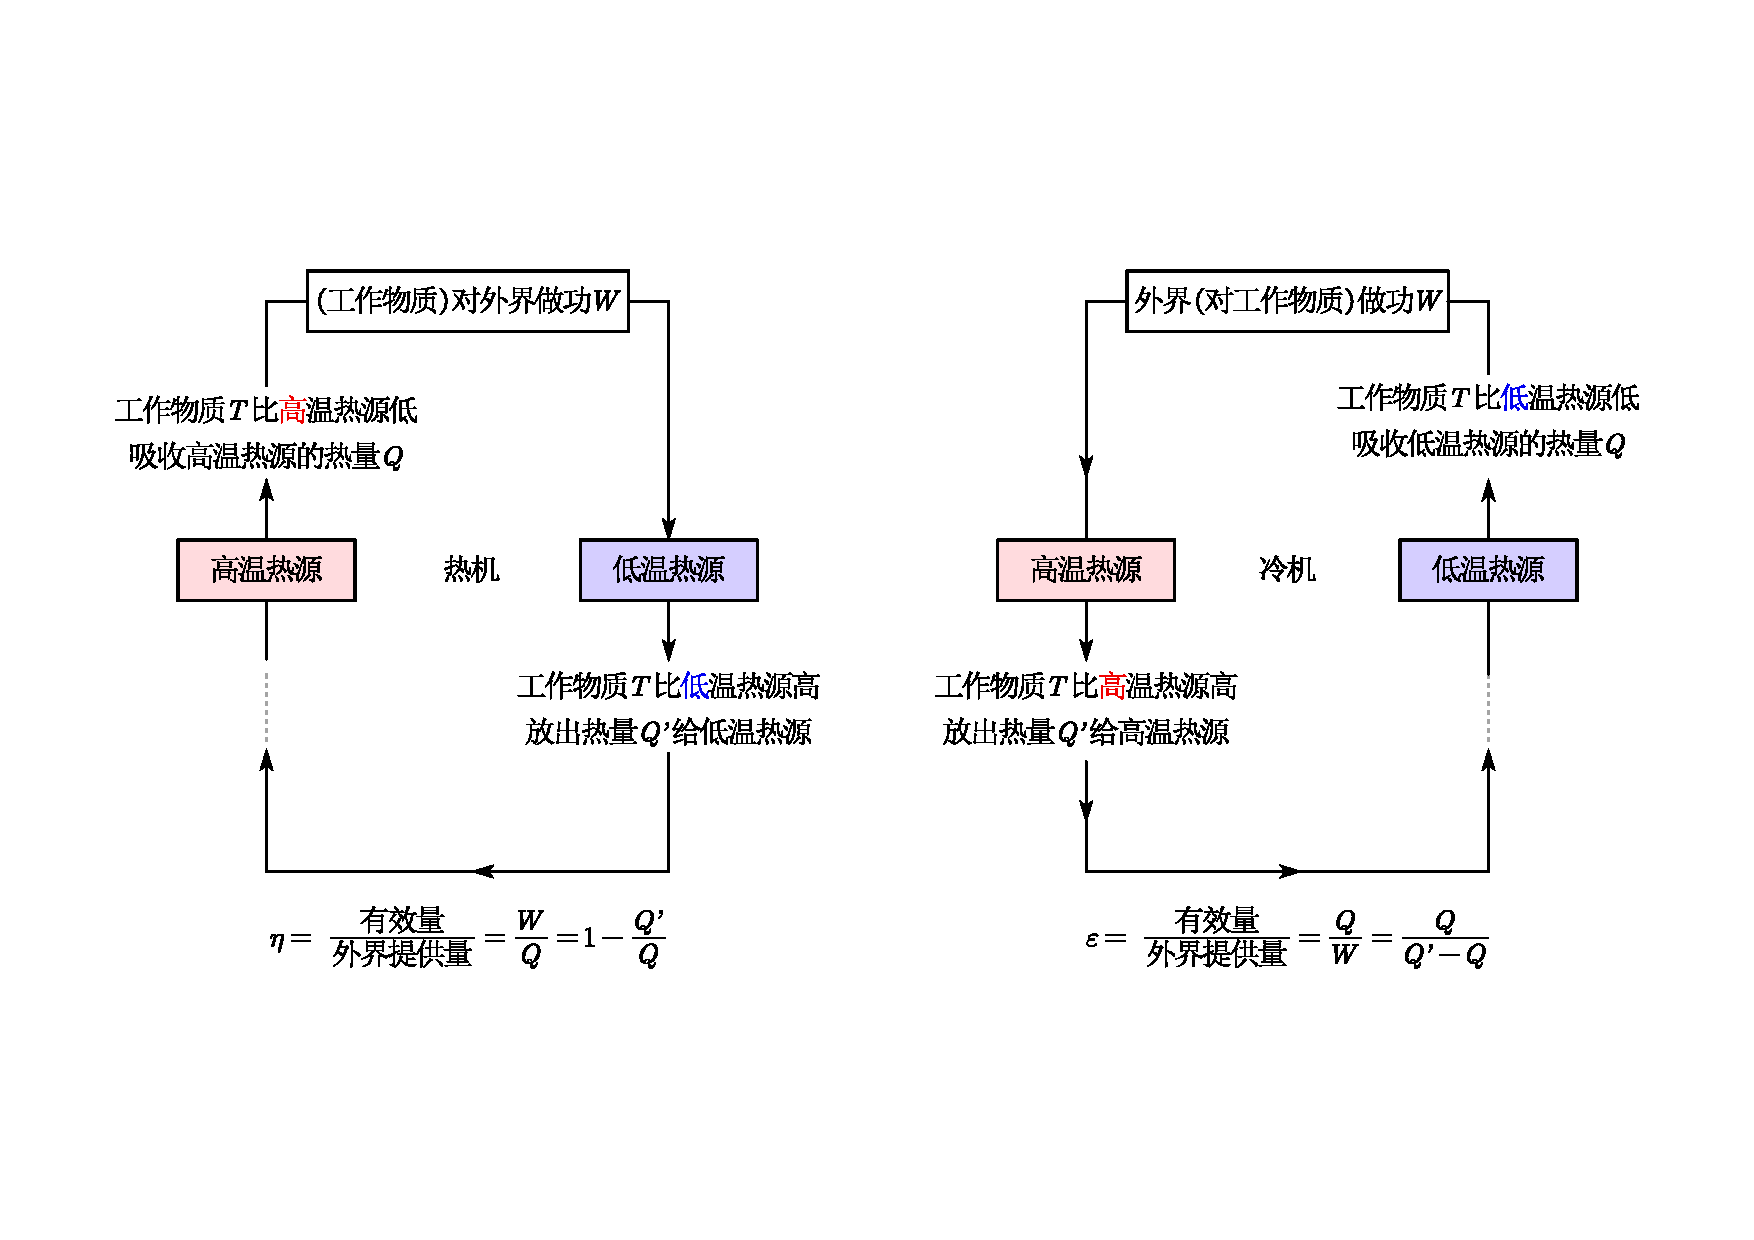
\includegraphics[width = \textwidth]{pic/热机冷机示意图.pdf}
    \caption{热机冷机示意图}
\end{figure}
热机从高温热源吸收热量,对外做功,并将将剩下的热量返还给低温热源;冷机从低温热源吸收热量,对外做功,并将剩下的热量返还给高温热源。
\subsubsection{卡诺定理:}
\ding{172}\ 一对高低温热源之间的可逆热机效率$\eta$仅取决于温度$T_2$、$T_1$,与热机过程无关。\par
\ding{173}\ 不可逆热机的效率$\eta' \le $可逆热机效率$\eta$。
{\par\color{gray}\small 只有无耗散的准静态过程才是可逆过程,其它一切过程(包括所有实际过程)都是不可逆过程。但是,目前所接触到的几乎所有问题,都是近似为可逆过程来计算。}\par
推论:可逆卡诺热机效率、卡诺制冷机制冷系数为(一对高低温热源间理论最高效率):
\begin{equation}
    \eta = \frac{T_1 - T_2}{T_1} = \frac{\Delta T}{T_{\text{高}}}\ ,\ \ \varepsilon = \frac{T_2}{T_1 - T_2} =\frac{T_{\text{低}}}{\Delta T} = \frac{1}{\eta} -1
\end{equation}

https://www.zhihu.com/question/22702847?utm\_id=1919810 \par


\subsubsection{内燃机、制冷机:}
提高热机效率的实际途径是提高高温热源的温度,由此产生了内燃机。将低温热源的热量转移到高温热源的设备称为制冷(或制热)机。\par
\ding{172}\ 奥托循环:由两个绝热过程和两个等体过程组成。
\begin{equation}
    \eta_A = 1 - \frac{1}{r^{\gamma -1}}
\end{equation}

\par
\ding{173}\ 狄赛尔循环:由两个绝热过程、一个等体过程和一个 等压过程组成。
\begin{equation}
    \eta_D =1- \frac{\rho^{\gamma} -1}{\gamma(\rho -1) r^{\gamma -1}}
\end{equation}
{\color{gray}\small $r = \frac{V_1}{V_2}$为体积压缩比,$\rho = \frac{V_1}{V_2}$为定压膨胀比。}
\chapter{热力学第二定律、第三定律}
\section{可逆、不可逆过程}
\subsubsection{热力学第二定律:}
\ding{172}\ 克劳修斯表述:不可能将热量从低温物体传递到高温物体而不产生任何其它影响。\par
\ding{173}\ 开尔文表述:不可能从单一热源吸收热量使之完全转化为有用功而不产生其它影响。\par
\ding{174}\ 熵增原理:孤立系统熵值永不减小(可逆时不变,不可逆时增大)。\par
{\par\color{gray}\small
孤立系统发生的过程都为绝热过程,本质是系统经绝热过程由一状态达到另一状态,熵不减小。也可表述为:热力学系统从一个平衡态经绝热过程到达另一个平衡态, 它的熵永不减少。若过程可逆,则其熵不变;若过程不可逆,则其熵增加。
\par}

\ding{175}\ 克劳修斯不等式(数学表述):
\begin{gather}
    \oint \frac{\mathrm{d}Q}{\, T\, } \le 0\ ,\ \ 
    \mathrm{d}S \ge \frac{\mathrm{d}Q}{T}
\end{gather}
{\color{gray}\small 当且仅当过程可逆时取等(实际过程都为不可逆过程但可近似为可逆过程)。闭合环路积分为0,说明被积量是某个函数的全微分(即为熵S)。另外,第二类永动机即为其逆否命题:能够从单一热源吸收热量将其全部转换为有用功而不产生任何其他影响的机械。}

\subsubsection{状态方程与内能、焓的关系:}
\ding{172}\ 内能$U$与状态方程:
\begin{equation}
    \left(\frac{\partial U}{\partial V} \right)_T = T \left(\frac{\partial p}{\partial T}\right)_V - p =p\left(\beta T -1\right)
\end{equation}
\par
\ding{173}\ 焓$H$与状态方程:
\begin{equation}
    \left(\frac{\partial H}{\partial p} \right)_T = -T \left(\frac{\partial V}{\partial T}\right)_p + V = V\left( 1- \alpha T\right)
\end{equation}
{\color{gray}\small 其中$\beta$为等体压强系数,$\alpha $为等压膨胀系数。证明详见 5.3 节}
\section{熵与熵变}
\subsubsection{熵定义:}
对\textcolor{red}{可逆过程} i 至 j,定义熵变为: 
\begin{equation}
    \mathrm{d}S = \frac{\mathrm{d}Q}{\,T\,} \ ,\ \ \Delta S = S_j -S_i  = \int_{i}^{j}\frac{\mathrm{d}Q}{\,T\,}
\end{equation}\par
{\par\color{gray}\small
上面我们仅定义了可逆过程下的熵微分,也即定义了可逆过程下的熵函数,可以用等号来描述。熵是态函数,只要过程可逆,无论如何从状态 i 达到状态 j,其熵变都相同。对于不可逆过程,可以证明其熵微分$\mathrm{d}S > \frac{\mathrm{d}Q}{\,T\,}$,一般只能用不等式描述。
\par}

\subsubsection{熵与熵变的计算:}
\noindent\ding{172}\ 熵的微分定义:
\begin{gather}
    \mathrm{d}S = \frac{\mathrm{d}Q}{T}\ \ \text{\color{gray}\small (可逆过程)}\ , \ \ \mathrm{d}S > \frac{\mathrm{d}Q}{T}\ \ \text{\color{gray}\small (不可逆过程)}
    \\
    \mathrm{d}S = \frac{C_V}{T}\mathrm{d}T + \beta p \mathrm{d}V= \frac{C_p}{T}\mathrm{d}T -\alpha V \mathrm{d}p  = \frac{C_V}{p} \mathrm{d}p + \frac{C_p}{V}\mathrm{d}V
\end{gather}
\noindent\ding{173}\ 理想气体的熵函数与熵变:
\begin{gather}
    \Delta S(T,V) = C_V\ln \left(\frac{T}{T_0}\right) + \nu R \ln \left(\frac{V}{V_0}\right)  \\
    \Delta S(T,p) = C_p\ln \left(\frac{T}{T_0}\right) - \nu R \ln \left(\frac{p}{p_0}\right) \\
    \Delta S = C_V \ln \left( \frac{p}{p_0}\right) + C_p \ln \left(\frac{V}{V_0}\right)\ \ \ {\color{red}\text{待定!!!}}
\end{gather}
{\par\color{gray}\small
{\color{red}掌握推导},并注意两式为一加一减。另外,计算{\color{red}自由膨胀过程 ($Q= 0, W=0, T=T_0$)} 的熵变时,可以设计等温过程,也可设计绝热+等体过程。
\par}

\begin{graybox}
\textbf{上式的证明:}\\
\textbf{(1)}
\begin{align*}
    \mathrm{d}S(T,V) 
    &= \left(\frac{\partial S }{\partial T }\right)_{V}\mathrm{d}T + \left(\frac{\partial S}{\partial V}\right)_{T}\mathrm{d}V \\
    &=  \frac{C_V}{T}\mathrm{d}T + \left(\frac{\partial p }{\partial T }\right)_{V}\mathrm{d}V\ \ \ {\color{gray}\text{(热容关系,Maxwell关系)}}  \\
    & = \frac{C_V}{T}\mathrm{d}T + \frac{\nu R}{V}\mathrm{d}V\ \ \ {\color{gray}\text{(理想气体)}}  \\
    \Longrightarrow \Delta S &= C_V\ln \left(\frac{T}{T_0}\right) + \nu R \ln \left(\frac{V}{V_0}\right)
\end{align*}
\textbf{(2)}
\begin{align*}
    \mathrm{d}S(T,p) 
    &= \left(\frac{\partial S }{\partial T }\right)_{p}\mathrm{d}T + \left(\frac{\partial S}{\partial p}\right)_{T}\mathrm{d}p \\
    &=  \frac{C_p}{T}\mathrm{d}T {\ \color{red} -\ } \left(\frac{\partial V }{\partial T }\right)_{p}\mathrm{d}p\ \ \ {\color{gray}\text{(热容关系,Maxwell关系)}}  \\
    & = \frac{C_p}{T}\mathrm{d}T {\ \color{red} -\ } \frac{\nu R}{p}\mathrm{d}p\ \ \ {\color{gray}\text{(理想气体)}}  \\
    \Longrightarrow \Delta S &= C_p\ln \left(\frac{T}{T_0}\right) {\ \color{red} -\ } \nu R \ln \left(\frac{p}{p_0}\right)
\end{align*}
\textbf{(3)}
\begin{align*}
    \mathrm{d}S(V,p) 
    &= \left(\frac{\partial S }{\partial V }\right)_{p}\mathrm{d}V + \left(\frac{\partial S}{\partial p}\right)_{V}\mathrm{d}p \\
    &= 
\end{align*}
\end{graybox}
\ding{174}\ 理想气体多方过程:
\begin{equation}
    \Delta S =  C_n\ln\left(\frac{T}{T_0}\right)=\left(C_V + \frac{\nu R}{1-n}\right)\ln\left(\frac{T}{T_0}\right)  = \left(C_p - \nu R \frac{n}{n - 1} \right)\ln \left(\frac{T}{T_0}\right) 
\end{equation}
{\par\color{gray}\small
\ding{173}\ding{174}的结论要求满足理想气体状态方程、$C_p$或$C_V$随温度不变(真实气体一般不满足此条,回到积分步骤重新积分即可),\ding{175}还要认为$\beta = \frac{1}{T}$或$\alpha = \frac{1}{T}$。
$n=0$时等压,$n=1$时等温,$n=\gamma$时绝热,$n=+\infty$时等体。对真实气体(热容是温度的函数),需要使用熵微分式进行积分:
\begin{equation}
    \Delta S = \int \frac{C_V(T)}{T}\mathrm{d}T + \beta p \mathrm{d}V
\end{equation}
\par}
\noindent\ding{175}\ 气体混合过程:
\begin{equation}
    {\color{red}\Delta S_{\text{mix}} = - \nu R \sum_{i=1}^{k}c_i\ln c_i >0}
\end{equation}
{\par\color{gray}\small
其中$c_i = \frac{\nu_i}{\nu} = \frac{\nu_i}{\sum_{i=1}^{k}\nu_i}$为气体浓度占比。
\par}
\noindent\ding{176}\ 相变过程:
\begin{equation}
    \Delta S = \int \frac{\mathrm{d}Q}{T} = \frac{\Delta Q}{T} =  \frac{\Delta U}{T} =  \frac{\Delta H}{T}
\end{equation}
{\par\color{gray}\small
上式要求相变过程在恒温恒压条件下进行、可近似为可逆过程,且环境的熵变也用上式计算。
\par}

\begin{graybox}
    \textbf{熵微分式的证明:}\\
    $S = S(T,V)$时,可推得:
    \begin{align*}
        \mathrm{d}S &= \frac{1}{T}\mathrm{d}Q = \frac{1}{T}\left[\mathrm{d}U - \mathrm{d}(W)\right]\\
        & = \frac{1}{T}\left[  \left(\frac{\partial U}{\partial V} \right)_T\mathrm{d}V + \left(\frac{\partial U}{\partial T} \right)_V\mathrm{d}T   + p\mathrm{d}V\right]\\
        &= \frac{1}{T} \left[ p(\beta  T-1)\mathrm{d}V+ C_V\mathrm{d}T + p\mathrm{d}V \right] \ \ \ (\text{内能与状态参量的关系})\\
        & = \frac{1}{T}\left[ \beta  pT\mathrm{d}V+ C_V\mathrm{d}T \right] =  \frac{C_V}{T}\mathrm{d}T + \beta  p \mathrm{d}V
    \end{align*}\par
    $S = S(T,p)$时,可推得:
    \begin{align*}
        \mathrm{d}S &= \frac{1}{T}\mathrm{d}Q 
        = \frac{1}{T}\left[\mathrm{d}U - \mathrm{d}(W)\right]
        = \frac{1}{T}\left[ \mathrm{d}H - \mathrm{d}(pV)   + p\mathrm{d}V\right]  \\
        &= \frac{1}{T}\left[ \left(\frac{\partial H}{\partial p} \right)_T\mathrm{d}T + \left(\frac{\partial H}{\partial T} \right)_p\mathrm{d}T - \mathrm{d}(pV)   + p\mathrm{d}V\right]\\
        &= \frac{1}{T} \left[ V(1- \alpha T)\mathrm{d}p+ C_p\mathrm{d}T - V\mathrm{d}p \right] \ \ \ (\text{焓与状态参量的关系})\\
        & = \frac{1}{T}\left[   C_p\mathrm{d}T - \alpha TV\mathrm{d}p \right] = \frac{C_p}{T}\mathrm{d}T - \alpha V\mathrm{d}p
    \end{align*}\par
    其中$\beta = \frac{1}{p}\left(\frac{\partial p}{\partial T} \right)_V = \frac{\nu R}{pV}\ \text{(理想气体)}$ 为等体压强系数,$\alpha= \frac{1}{V}\left(\frac{\partial V}{\partial T} \right)_p = \frac{\nu R}{pV} \ \text{(理想气体)}$为等压膨胀系数。
\end{graybox}
    

\subsubsection{熵增原理:}
对所有的绝热过程,有:
\begin{equation}
    \Delta S_{\text{绝热}} \ge  0
\end{equation}
{\par\color{gray}\small
当且仅当过程可逆时取等。孤立系统中发生的所有过程均为绝热过程,因此必有$S_{\text{孤立}} \ge 0$
\par}

\subsubsection{微观熵(玻尔兹曼熵):}
设系统微观状态数为$\Omega$,定义微观熵:
\begin{equation}
    S = k\ln \Omega
\end{equation}
{\par\color{gray}\small
其中 $k$为比例系数。可以证明,对于可逆过程,微观熵(玻尔兹曼 熵)与宏观熵(克劳修斯熵)完全相同。
\par}

\section{自由能、自由焓、化学势与热力学方程}

\subsubsection{热力学基本方程:}
联立热一与热二(熵的定义),有热力学基本方程($T\mathrm{d}S$方程):
\begin{align*}
    T\mathrm{d}S &= \mathrm{d}U +p\mathrm{d}V  
    = \mathrm{d}H - V\mathrm{d}p \\
    (\text{联立}&\text{自由焓$F$和吉布斯自由能$G$定义的全微分})\\
    S\mathrm{d}T& = -\mathrm{d}F - p\mathrm{d}V = -\mathrm{d}G - V\mathrm{d}p 
\end{align*}


\subsubsection{热力学基本关系:}
热力学基本方程:
\begin{table}[H]
    \centering
    \begin{tabular}{cccc} 
    \toprule
    名称 & 定义 & 热力学基本方程(可逆) & 基本方程(不可逆)  \\
    \midrule
    内能$U$ & $U = U(T,V)$ & $\mathrm{d}U = T\mathrm{d}S -p\mathrm{d}V $ &  $\mathrm{d}U < T\mathrm{d}S -p\mathrm{d}V $ \\
    焓$H$ & $H = U+pV$ & $\mathrm{d}H = T\mathrm{d}S  + V\mathrm{d}p$ &$\mathrm{d}H < T\mathrm{d}S  + V\mathrm{d}p$\\
    自由能$F$ & $F = U-TS$ & $\mathrm{d}F = -S\mathrm{d}T-p\mathrm{d}V$ & $\mathrm{d}F < -S\mathrm{d}T-p\mathrm{d}V$  \\
    自由焓$G$ & $G = H - TS$ & $\mathrm{d}G = -S\mathrm{d}T + V\mathrm{d}p$ & $\mathrm{d}G < -S\mathrm{d}T + V\mathrm{d}p$  \\
    \bottomrule
    \end{tabular}
\end{table}
(等温等体)最大功原理: $\mathrm{d}W' \le -\mathrm{d}F$,(等温等压)最大非体积功: $\mathrm{d}W'' \le -\mathrm{d}G$

{\par\color{gray}\small
上表中的不等式当且仅当过程可逆时取等,在实际的题目中,除非题目特别指明,一般都近似为可逆过程处理。另外,{\color{red}在等温等体条件下,系统热平衡态对应自由能$F$极小,在等温等压条件下,系统热平衡态对应自由焓(吉布斯自由能) $G$极小。}
\par}
八个偏导数关系(由热力学基本方程导出):
\begin{table}[H]
    \centering
    \begin{tabular}{ccc} 
    \toprule
    名称 & 偏导1 & 偏导2  \\
    \midrule
    $U = U(S,V)$ & $\left(\frac{\partial U}{\partial S}\right)_V = T$ & $\left(\frac{\partial U}{\partial V}\right)_S =-p $ \\
    $H = H(S,p)$ & $\left(\frac{\partial H}{\partial S}\right)_p = T$ & $\left(\frac{\partial H}{\partial p}\right)_S = V $ \\
    $F = F(T,V)$ & $\left(\frac{\partial F}{\partial T}\right)_V = -S$ & $\left(\frac{\partial F}{\partial V}\right)_T = -p$ \\
    $G = G(T,p)$ & $\left(\frac{\partial G}{\partial T}\right)_p = -S$ & $\left(\frac{\partial G}{\partial p }\right)_T = V$ \\
    \bottomrule
    \end{tabular}
\end{table}


两个热容关系:
\begin{gather}
    C_V = \left(\frac{\partial U }{\partial T }\right)_{V} =  \left(\frac{\partial U }{\partial S }\right)_{V} \left(\frac{\partial S }{\partial T }\right)_{V} = T \left(\frac{\partial S }{\partial T }\right)_{V}
    \Longrightarrow {\color{red}\left(\frac{\partial S}{\partial T}\right)_V = \frac{C_V}{T} }
    \\
    C_p = \left(\frac{\partial H }{\partial T }\right)_{p} =  \left(\frac{\partial H }{\partial S }\right)_{p} \left(\frac{\partial S }{\partial T }\right)_{p} = T \left(\frac{\partial S }{\partial T }\right)_{p}
    \Longrightarrow  {\color{red}\left(\frac{\partial S}{\partial T}\right)_p =\frac{C_p}{T} }
\end{gather}

Maxwell关系:
\begin{gather}
    {\color{red}
    \left(\frac{\partial S}{\partial V}\right)_T =\left(\frac{\partial p}{\partial T}\right)_V\ ,\ \ \left(\frac{\partial S}{\partial p}\right)_T = -\left(\frac{\partial V}{\partial T}\right)_p
    }
    \\
    \left(\frac{\partial V}{\partial S}\right)_p = \left(\frac{\partial T}{\partial p}\right)_S  \ ,\ \  \left(\frac{\partial p}{\partial S}\right)_V = - \left(\frac{\partial T}{\partial V}\right)_S
\end{gather}
{\par\color{gray}\small
由八个偏导数关系导出(成对一阶偏导分别求二阶导)。可理解为两个偏导,取倒数后得到一共四个,但要注意右下角标发生了变化(都是对方分母量不变)。
\par}

\subsubsection{内能、焓与状态方程:}
\noindent\ding{172} $S = S(T,V)$导出内能$U$与状态方程$p,V,T$的关系,即$\mathrm{d}U = \mathrm{d}U(T,V)$:
\begin{gather}{\color{red}
    \left(\frac{\partial U }{\partial V }\right)_{T} = T \left(\frac{\partial p }{\partial T }\right)_{V} -p}
    \Longrightarrow 
    \mathrm{d}U(T,V) = C_V\mathrm{d}T + \left[ T \left(\frac{\partial p }{\partial T }\right)_{V} -p\right]\mathrm{d}V 
\end{gather}
\begin{graybox}
\textbf{上式的证明:}
\begin{align*}
    \text{热容关系+Maxwell关系:}&\mathrm{d}S = \left(\frac{\partial S }{\partial T }\right)_{V}\mathrm{d}T + \left(\frac{\partial S }{\partial V }\right)_{T}\mathrm{d}V=\frac{C_V}{T}\mathrm{d}T + \left(\frac{\partial p }{\partial T }\right)_{V}\mathrm{d}V\\ \label{ eq:S-T-V}
    \text{热力学基本方程:}&\mathrm{d}S =\frac{1}{T}\left[\mathrm{d}U\right] + \frac{p}{T}\mathrm{d}V = \frac{1}{T}\left[ \left(\frac{\partial U }{\partial T  }\right)_{V}\mathrm{d}T + \left(\frac{\partial U }{\partial V }\right)_{T}\mathrm{d}V \right] + \frac{p}{T}\mathrm{d}V \\ 
    &\ \ \ \ \ = \frac{C_V}{T}\mathrm{d}T + \frac{1}{T} \left[\left(\frac{\partial U }{\partial V }\right)_{T} + p\right]\mathrm{d}V\\ 
    \text{两式对比}\ &\Longrightarrow \left(\frac{\partial p }{\partial T }\right)_{V} = \frac{1}{T} \left[\left(\frac{\partial U }{\partial V }\right)_{T} + p\right] \\ 
    &\Longrightarrow \left(\frac{\partial U }{\partial V }\right)_{T} = T \left(\frac{\partial p }{\partial T }\right)_{V} -p
\end{align*}
\end{graybox}

\noindent\ding{173} $S = S(T,p)$导出焓$H$与状态方程$p,V,T$的关系,即$\mathrm{d}H = \mathrm{d}H(T,p)$:
\begin{equation}
    {\color{red}\left(\frac{\partial H }{\partial V }\right)_{T} = - T\left(\frac{\partial V }{\partial T }\right)_{p} +V}\Longrightarrow \mathrm{d}H = C_p\mathrm{d}T + \left[- T\left(\frac{\partial V }{\partial T }\right)_{p} +V\right]\mathrm{d}p 
\end{equation}
\begin{graybox}
\textbf{上式的证明:}
\begin{align*}
    \text{热容关系+Maxwell关系:}&\mathrm{d}S = \left(\frac{\partial S }{\partial T }\right)_{p}\mathrm{d}T + \left(\frac{\partial S }{\partial p }\right)_{T}\mathrm{d}p=\frac{C_p}{T}\mathrm{d}T - \left(\frac{\partial V }{\partial T }\right)_{p}\mathrm{d}p\\ 
    \text{热力学基本方程:}&\mathrm{d}S =\frac{1}{T}\left[\mathrm{d}H\right] - \frac{V}{T}\mathrm{d}p = \frac{1}{T}\left[ \left(\frac{\partial H }{\partial T  }\right)_{p}\mathrm{d}T + \left(\frac{\partial H }{\partial V }\right)_{T}\mathrm{d}V \right] - \frac{V}{T}\mathrm{d}p \\ 
    &\ \ \ \ \ = \frac{C_p}{T}\mathrm{d}T + \frac{1}{T} \left[\left(\frac{\partial H }{\partial V }\right)_{T} - V\right]\mathrm{d}p\\ 
    \text{两式对比}\ &\Longrightarrow - \left(\frac{\partial V }{\partial T }\right)_{p} =  \frac{1}{T} \left[\left(\frac{\partial H }{\partial V }\right)_{T} - V\right]\\ 
    &\Longrightarrow \left(\frac{\partial H }{\partial V }\right)_{T} = - T\left(\frac{\partial V }{\partial T }\right)_{p} +V
\end{align*}
\end{graybox}

\subsubsection{化学势:}
上面的结论都是对于封闭系统($N = const$),对开放系统,我们引入化学势的概念:
\begin{equation*}
    \mu = \left(\frac{\partial G }{\partial N }\right)_{T,p}
\end{equation*}
{\par\color{gray}\small
相应的,会衍生出开放系统下的热力学基本方程,例如$T\mathrm{d}S = \mathrm{d}U + p\mathrm{d}V +\mu\mathrm{d}N$,它们可由$\mathrm{d}G = -S\mathrm{d}T +V\mathrm{d}p + \mu\mathrm{d}N$导出,这里不再赘述。\par
\par}
特别地,对所有单相物质,其吉布斯自由能$G$与粒子个数$N$成正比,因此$ \mu = \left(\frac{\partial G }{\partial N }\right)_{T,p} {\color{red}= \frac{G}{N}}$


\subsubsection{开放系统:}
\par\ding{172}\  化学势:$\mu = -\left(\frac{\partial G}{\partial N}\right)_{p,T}$\par
\ding{173}\  推论: $\mathrm{d}G \le -S\mathrm{d}T + V\mathrm{d}p +\mu \mathrm{d}N$  \par
\ding{174}\   开放系统基本方程:$T\mathrm{d}S = \mathrm{d}U + p\mathrm{d}V - \mu \mathrm{d}N$  \par
\ding{175}\   化学势:$\mu =\frac{G}{N}$  \par
{\par\color{gray}\small
对所有单相物质,化学势就是每个粒子所具有的自由焓(每个粒子所具有的吉布斯自由能)。
\par}

\subsubsection{不同系统的热平衡判据:}

\begin{table}[H]
    \caption{\textbf{不同系统的热平衡判据}}
    \centering
    \begin{tabular}{ccccccc} 
    \toprule
    系统条件& 原理 &方程 & 热平衡判据 \\
    \hline
    孤立 & 熵增原理 &$\mathrm{d}S \ge 0$ & $\mathrm{d}S=0$\\
    等温等体 & 自由能减小原理 & $\mathrm{d}F \le -S\mathrm{d}T - p\mathrm{d}V$  & $\mathrm{d}F = 0$\\
    等温等压 & 最大功原理 & $\mathrm{d}G \le -S\mathrm{d}T + V\mathrm{d}p $& $\mathrm{d}G = 0$ \\
    相平衡(等温等压) & 质量守恒 & $\mathrm{d}G = \mu_1 \mathrm{d}N_1 + \mu_2\mathrm{d}N_2 = 0$& $\mu_1 = \mu_2$ \\
    \bottomrule
    \end{tabular}
\end{table}
{\par\color{gray}\small
对等温等体、等温等压,我们分别有两个最大非体积功推论:$\mathrm{d}W'\le -\mathrm{d}F$,$\mathrm{d}W'' \le -\mathrm{d}G$。

\par}


\section{热力学第三定律}
\subsubsection{熵的标准参考点:}

{\par\color{gray}\small
能斯特定理表明,在绝对零度的条件下,任何凝聚物质系统的熵的差值都为 0。这就是说,确实存在使任何物质的熵都相同的状态。因此对于熵,存在标准参考点。像上式,选取绝对零度为熵的零点,称为普朗克熵。
\par}
\subsubsection{热力学第三定律:}
\ding{172} 常见表述:
不可能通过有限步骤把一个物体的温度冷却到绝对零度。
{\par\color{gray}\small
但不排除通过一些手段无限接近绝对零度的可能性。
\par}
\ding{173} 普朗克熵表述:任意纯物质在绝对温度为0时的熵为0,即$\lim_{T\rightarrow 0} S(T) = 0$\par

\chapter{液态系统的性质}
\section{液体的性质}
液体的分类,微观结构与研究方法详见课本,这里不再赘述。
\subsubsection{液体黏度}
对液体的(剪切)黏度,我们有费朗科尔-安德逊公式:
\begin{equation}
\eta = \eta_0e^{\frac{E_a}{k_BT}}
\end{equation}
{\par\color{gray}\small
其中$\eta_0 = \underset{{T\rightarrow+\infty}}{\lim} \eta(T)$为常量,$E_a$为液体分子激活能,它们都由系统的内禀性质决定。
\par}

\subsubsection{液体热容量:}
液体的定压热容$C_p^{(l)}$与固体定压热容相近,但定体热容不确定。
\ding{172}定压热容$C_p^{(l)}$:\par
\begin{equation}
    C_p^{(l)} = C_p^{(s)} = 3\nu R\ \ {\color{gray}(t=0, r=0, s=3)} 
\end{equation}
\par\ding{173}定体热容$C_V^{(l)}$:\par
\begin{gather}\label{液体定体热容}
    C_p - C_V = T\left(\frac{\partial p}{\partial T}\right)_V\left(\frac{\partial V}{\partial T}\right)_p = VT\frac{\alpha^2}{\kappa}\ \ \text{\color{gray}(对任意系统成立)}\\
    \Longrightarrow C_V  = 3\nu R  - T\left(\frac{\partial p}{\partial T}\right)_V\left(\frac{\partial V}{\partial T}\right)_p
\end{gather}
{\par\color{gray}\small
其中$\alpha$为系统(可以是固、液、气)的体膨胀系数,$\kappa = \kappa_T$为等温压缩系数。对于液体,其体膨胀系数$\alpha$和等温压缩系数$\kappa$是复杂的、不断变化的函数,因此不仅$C_p^{(l)} \ne C_p^{(s)} $,而且$C_p^{(l)} - C_p^{(s)} \ne \text{const}$。
\par}

\begin{graybox}
\textbf{公式 \ref{液体定体热容} 的证明:}
\begin{align*}
    C_V &= \left(\frac{\partial Q}{\partial T}\right)_V = \left(\frac{\partial U}{\partial T}\right)_V\ \ {\color{gray} \mathrm{d}U = \mathrm{d}Q -p\mathrm{d}V,\ \mathrm{d}V=0} \\ 
    C_p &= \left(\frac{\partial Q}{\partial T}\right)_p  =  \left(\frac{\partial H}{\partial T}\right)_p  \ \ {\color{gray} \mathrm{d}U = \mathrm{d}Q -p\mathrm{d}V ,\ H = U+pV,\ \mathrm{d}H = \mathrm{d}U + p\mathrm{d}V + V\mathrm{d}p (\mathrm{d}p=0)}\\ 
    &= \left(\frac{\partial (U+pV)}{\partial T}\right)_p =  \left(\frac{\partial U}{\partial T}\right)_p + p \left(\frac{\partial V}{\partial T}\right)_p \\ 
    &= \left[ \left(\frac{\partial U}{\partial T}\right)_V  + \left(\frac{\partial U}{\partial V}\right)_T\left(\frac{\partial V}{\partial T}\right)_p  \right]  + p \left(\frac{\partial V}{\partial T}\right)_p\ \  {\color{gray}U = U(T,V(T,p)),\ \text{由复合函数求导}}
\end{align*}
\begin{align*}
    &= \left(\frac{\partial U}{\partial T}\right)_V + \left[ \left(\frac{\partial U}{\partial V}\right)_T +p \right]\left(\frac{\partial V}{\partial T}\right)_p\\
    &= \left(\frac{\partial U}{\partial T}\right)_V + \left[ T\left(\frac{\partial p}{\partial T}\right)_V\right]\left(\frac{\partial V}{\partial T}\right)_p\ \ {\color{gray}\text{内能与状态方程关系} \left(\frac{\partial U}{\partial V} \right)_T = T \left(\frac{\partial p}{\partial T}\right)_V - p}\\
    &\Longrightarrow C_p - C_V =  T\left(\frac{\partial p}{\partial T}\right)_V\left(\frac{\partial V}{\partial T}\right)_p
\end{align*}
\end{graybox}

\subsubsection{液体输运性质:}
\par\ding{172}\ 黏滞现象:
\begin{equation}
    f = - \eta \frac{\mathrm{d}v}{\mathrm{d}z}\ , \ \ \eta = \eta_0e^{\frac{E_a}{k_BT}}
\end{equation}\par
\ding{173}\  热传导现象:
液体的热传导依靠分子间碰撞进行,而碰撞极小,因此大多热导性不好(导热系数$\kappa$低)。  \par
\ding{174}\   扩散现象:
\begin{equation}
    \boldsymbol{j}_N = -D\nabla n\ ,\ \ D = D_0e^{-\frac{E_a}{k_BT}}
\end{equation}  \par
{\par\color{gray}\small
其中$\eta_0 = \underset{{T\rightarrow+\infty}}{\lim} \eta(T)$,$D_0 = \underset{{T\rightarrow+\infty}}{\lim} D(T)$,$E_a$称为液体分子的激活能(液体分子相互作用势阱深度的平均值)。注意$\eta$的指数中无负号,而$D$的指数中有负号。
\par}

\subsubsection{液体表面性质:}
\par\ding{172}\ 表面张力:
\begin{equation}
    \mathrm{d}f_s = \sigma\mathrm{d}l\ ,\ \ \mathrm{d}W = \sigma \mathrm{d}A
\end{equation} \par
\ding{173}\  表面张力系数的确定:
\begin{equation}
    \sigma = (1 - \xi )\frac{L_m}{N_A}\left(\frac{\rho N_A}{\mu}\right)^{\frac{2}{3}}
\end{equation}   \par
{\par\color{gray}\small
$\sigma = \frac{\mathrm{d}W}{\mathrm{d}A}$称为表面张力系数,$\mathrm{d}A$表示液体的面积增量微元;$\xi$为相对粒子数密度(液体表面层粒子数密度占内部粒子数密度的比值,多数为$\xi \approx 0.7$),$L_m$为液体摩尔汽化热,$\rho$为气体密度,$\mu$为液体摩尔质量。\par
注意:液膜有两个表面,因此表面积发生变化时,表面能变化(即外界做功量) ${\color{red}\mathrm{d}F_S = 2\sigma \mathrm{d}A}$
\par}

\subsubsection{表面能与表面内能:}
表面能$F_S$即表面自由能,表面内能$U_S$,表面内能密度$u_S$,且有:
\begin{equation*}
    {\color{red}F_S = \sigma A}\ ,\ \ U_S = F_S -TA \left(\frac{\partial \sigma }{\partial T }\right)_{A}\ ,\ \ u_S = \sigma - T \left(\frac{\partial \sigma }{\partial T }\right)_{A}
\end{equation*}
{\par\color{gray}\small
其中$A$为表面面积,$\sigma$为表面张力系数。\par
注意:$F_S$仅为表面自由能,总自由能由$F_G = U-TS$和$F_S = \sigma A$构成,例如 {\color{red}$\Delta W =  \Delta F = \Delta F_G + \Delta F_S$}。
\par}
\begin{graybox}
\textbf{上式的证明:}\\
将热力学基本公式与$F = \sigma A$联立:
\begin{align*}
    \mathrm{d}F(A,T)  = \mathrm{d}W - T\mathrm{d}S &= \sigma\mathrm{d}A - S\mathrm{d}T \ \ \text{\color{gray}(由热力学基本公式)} \\
    \mathrm{d}F(A,T)  = \left(\frac{\partial F }{\partial A }\right)_{T}\mathrm{d}A + \left(\frac{\partial F }{\partial T }\right)_{A}\mathrm{d}T &= \sigma \mathrm{d}A + A \left(\frac{\partial \sigma }{\partial T }\right)_{A}\mathrm{d}T \ \ \text{\color{gray}(由$F = F(A,T) = \sigma A$)} 
\end{align*}
两式对比即得{\color{red}$S = -  A \left(\frac{\partial \sigma }{\partial T }\right)_{A}$},因此:
\noindent\begin{equation*}
    F_S = \sigma A\ ,\ \ U_S = \sigma A -TA \left(\frac{\partial \sigma }{\partial T }\right)_{A}
\end{equation*}
\end{graybox}

\subsubsection{拉普拉斯公式:}
任意弯曲液面内外的压强差可表示为:
\begin{equation}
    \Delta p = \sigma(\frac{1}{R_1} + \frac{1}{R_2})
\end{equation}
{\par\color{gray}\small
其中$R_1$,$R_2$为弯曲液面上的两个正截口的曲率半径(曲率中心在液体内$R>0$,液体外$R<0$),而正截口指包含曲面法线的平面与曲面的交线。注意,液膜有两个表面,因此内外气体压强差为{\color{red}$\Delta p =\frac{2\sigma}{R}+\frac{2\sigma}{R} = \frac{4\sigma}{R}$}。例如,液泡膜和水滴的情况不同,液泡膜是$\Delta p = \frac{4\sigma}{R}$,水滴是$\Delta p = \frac{2\sigma}{R}$。
\par}

\section{润湿与毛细现象}
\subsubsection{润湿现象:}
\par\ding{172}\ 接触角:液固接触点(或液液接触点)液面的切线与液体内部两物质表面切线之间的夹角称为接触角。    \par
\ding{173}\  润湿程度:
\begin{equation}
    \begin{cases}
        \text{完全润湿} & \text{ if }\  \theta=0 \\
        \text{部分润湿} & \text{ if }\  \theta \in (0,\frac{\pi}{2} ) \\
        \text{部分不润湿} & \text{ if }\  \theta \in [\frac{\pi }{2},\pi  )\\
        \text{完全不润湿} & \text{ if }\ \theta = \pi
    \end{cases}
\end{equation}   \par
\ding{174}\  液液接触角:
\begin{equation}
    \cos\theta = \frac{\sigma_{13}^2 - (\sigma_{12} +\sigma_{23})^2}{2\sigma_{12}\sigma_{23}}
\end{equation} 
{\par\color{gray}\small
在液体1与空气3的交界面上有一滴液体2,在三者交界处取一线元$\mathrm{d}l$,由力学平衡,作平方后相加即得。两种介质交界面处,若两种都不为真空,则表面张力系数是相对的,因此写作$\sigma_{ij}$或$\sigma_{ji}$。
\par} \par
\ding{175}\ 固液接触角:
\begin{equation}
    \cos \theta = \frac{\sigma_{13} - \sigma_{12}}{\sigma_{23}}
\end{equation}\par
\ding{176}\ 粗糙表面:
\begin{equation}
    \cos \theta' = r\cos\theta\ ,\ \ r \in [1,+\infty]
\end{equation}
\ding{177}\ 有气泡粗糙表面:
\begin{equation}
    \cos \theta' = f-1 + rf\cos\theta\ ,\ \ f \in [0,1],\ r \in [1,+\infty] 
\end{equation}
{\par\color{gray}\small
$\theta'$为粗糙面上的接触角,$r = \frac{\text{真实表面面积}}{\text{投影面积}} >1$为粗糙度,$0\le f\le 1$为投影面积中润湿部分的比值(全部润湿时$f=1$)。
\par}

\subsubsection{毛细现象:}

任意固定一高度为参考点(一般选取管外液体表明),设该点处液体压强为$p_0$,则我们有:
\begin{equation}
    {\color{red}\Delta p = \rho g h}
\end{equation}
{\par\color{gray}\small
其中$h$为高出参考点的高度,$\Delta p$由拉普拉斯定理得到。下面是三个具体例子:
\par}

{\par\color{gray}\small
\par\ding{172}\  直立圆柱毛细管:
\begin{equation*}
    h = \frac{2\sigma \cos\theta}{\rho gr}
\end{equation*}  
{\par\color{gray}\small
$\sigma$为液体与空气间的表面张力系数,$r$为毛细管半径,$\theta$为固液接触角。
\par}\par
\ding{173}\   两竖直平行板:  \par
{\par\color{gray}\small
\begin{equation*}
    h = \frac{2\sigma \cos\theta}{\rho gr}
\end{equation*}
\par}
\ding{174}\  两相交平面:
\begin{equation*}
    h= h = \frac{2\sigma \cos\theta}{\rho g \varphi x}
\end{equation*}   \par
\par}


\chapter{相变与复相平衡}
\subsubsection{相与相平衡:}
在没有外界影响下,被一定边界包围的,具有确定并且均匀的物理和化学性质的一个系统(或系统的一部分)所处的状态称为物质的一个相。一般地,平衡态稳定条件可以表示为:
\begin{equation}
    \frac{\partial \mu }{\partial N } >0\ ,\ \ C_V >0\ ,\ \ \kappa_S \ge 0
\end{equation}
{\par\color{gray}\small
其中$\kappa_S = - \frac{1}{V}\left(\frac{\partial V}{\partial p }\right)_{S}$为绝热压缩系数(即等熵压缩系数)。
\par}
又对于理想气体,我们有$\kappa_S = \frac{1}{\gamma}\kappa_T$,后者为等温压缩系数,因此平衡条件等价于:
\begin{equation}
    \frac{\partial \mu }{\partial N } >0\ ,\ \ C_V >0\ ,\ \ \kappa_T \ge 0
\end{equation}
\subsubsection{相变:}
由相平衡,相变满足方程:
\begin{equation}
    \frac{\mathrm{d}p}{\mathrm{d}T} = \frac{S_{\beta,m} - S_{\alpha,m}}{V_{\beta,m}-V_{\alpha,m}}
\end{equation}
对不同级别的相变,我们有不同的推论。
\subsubsection{一级相变:}
固液、固气、液气相变都是一级相变,对\textcolor{red}{一级相变},我们有克拉伯龙方程:
\begin{equation}
    \frac{\mathrm{d} p}{\mathrm{d}T} = \frac{\Lambda_m}{T(V_{\beta,m}-V_{\alpha,m})}
\end{equation}
{\par\color{gray}\small
其中$\Lambda_m$为摩尔相变潜热(例如摩尔熔解热、摩尔汽化热),在一级相变中$\Lambda_m = T(S_{\beta,m} - S_{\alpha,m})$,$T$为相变温度(如熔解稳定)$V_{\beta,m}$为$\beta$相的摩尔体积,$V_{\alpha,m}$为$\alpha$相的摩尔体积。\par
设$V_{\alpha,m}$可忽略且$\beta$可视为理想气体,则可以估算某温度区间的平均相变潜热:
\begin{equation*}
    \Lambda_m = R\frac{\frac{1}{p}\mathrm{d}p}{\frac{1}{T^2}\mathrm{d}T}\Longrightarrow \overline{\Lambda_m} = \frac{R(\ln p_1 - \ln p_2)}{\frac{1}{T_1} - \frac{1}{T_2}} =  R\ln(\frac{p_1}{p_2})\frac{T_1T_2}{T_1 - T_2}
\end{equation*}
当然,其实也可以用:
\begin{equation*}
    \Lambda_m = R\frac{\frac{1}{p}\mathrm{d}p}{\frac{1}{T^2}\mathrm{d}T} = \frac{RT^2}{p}\cdot \frac{\mathrm{d}p}{\mathrm{d}T}
\end{equation*}
注意:熔解热、液化热、汽化热都是指\textcolor{red}{单位质量}吸收/放出的热量,有 \textcolor{red}{ $l = \frac{\Lambda_m}{\mu}$}。
\par}

\subsubsection{二级相变:}
对于二级相变,我们有埃伦费斯特方程:
\begin{gather}
    \frac{\mathrm{d} p}{\mathrm{d}T} = \frac{C_{p,m,\beta} - C_{p,m,\alpha}}{TV_m(\alpha_\beta - \alpha_\alpha)}\\
    \frac{\mathrm{d} p}{\mathrm{d}T} = \frac{\alpha_\beta - \alpha_\alpha}{\kappa_{T,\beta} - \kappa_{T,\alpha}}
\end{gather}
{\par\color{gray}\small
其中$C_{p,m,\beta}, C_{p,m,\alpha}$为摩尔定压热容,$\alpha_\beta, \alpha_\alpha$为体膨胀系数,$\kappa_{T,\beta}, \kappa_{T,\alpha}$为等温压缩系数。结论的推导用到 Maxwell 偏导关系。
\par}







\newpage
\nocite{*}
\bibliography{re}
\addcontentsline{toc}{chapter}{参考文献}


\newpage
\appendix
\addcontentsline{toc}{chapter}{附录}
\titleformat{\section}{\large\centering\bfseries}{Apendix\thesection}{1em}{}
\titleformat{\subsection}{\normalsize\bfseries}{\thesubsection}{1em}{}

\section{常见物理常量表}
\begin{longtable}[H]{cccc}
    \caption{\textbf{常见物理常量数值}}\\
    \toprule
    名称 & 符号&  数值& 单位\\
    \midrule
    \endfirsthead
    % 这里是表格内容
    \bottomrule
    \endfoot

    \toprule
    \multicolumn{4}{c}{\textbf{续上表}}\\
    \midrule
    名称 & 符号&  数值& 单位\\
    \midrule
    \endhead
    % 这里是表格内容
    \bottomrule
    \endlastfoot
    阿伏伽德罗常量& $N_\text{A}$ & $6.02\times 10^{23}  $ & $\mathrm{mol}^{-1}$\\
    普适气体常量& $R=\frac{p_0V_m}{T_0} $& $8.31$& $\mathrm{J\cdot mol^{-1} \cdot K^{-1}}$\\
    普适气体常量& $R=\frac{p_0V_m}{T_0} $& $0.082$& $\mathrm{atm\cdot L\cdot mol^{-1} \cdot K^{-1}}$\\ 
    玻尔兹曼常量& $k_B=\frac{R}{N_A} $& $1.38\times10^{-23}$& $\mathrm{J\cdot K^{-1}}$\\
    大气压强& $p_0$& $1.01\times 10^5$& $\mathrm{Pa}$\\
    大气压强& $p_0$& $1$& $\mathrm{atm}$\\
    大气压强& $p_0$& $760$& $\mathrm{mmHg}$\\
    标准状况温度& $T_0$& $273.15$& $\mathrm{K}$\\
    空气平均摩尔质量& $\mu_{\text{air}}$& $29\times 10^{-3}$& $\mathrm{kg\cdot mol^{-1}}$
\end{longtable}

\end{document}